\documentclass[a4paper, 12pt]{report}
\usepackage[a4paper, top=1in, bottom=0.75in, left=1.25in, right=1in, headheight=15pt, headsep=0.25in]{geometry}
\usepackage{setspace}
\usepackage{titlesec}
\usepackage{graphicx}
\usepackage{caption}
\usepackage[labelfont=bf, textfont=normalfont]{caption}
\usepackage{fancyhdr}
\usepackage{indentfirst} 
\usepackage[x11names]{xcolor}
\usepackage{lipsum}
\usepackage{tikz}
\usepackage{eso-pic}
\usepackage{etoolbox}
\usepackage{newtxtext,newtxmath}
\usepackage[colorlinks=true, linkcolor=black, urlcolor=blue, citecolor=black]{hyperref}
\usepackage[authoryear]{natbib}
\usepackage{subfig}
\usepackage{cite}
\usepackage{float}
\usepackage{longtable}
\usepackage{multirow}
\usepackage{enumitem}
\usepackage{amsmath}
\usepackage{algorithm}
\usepackage{algpseudocode}
\usepackage{listings}
\usepackage{fontspec}
\usepackage{ragged2e}
\makeatletter
\@ifundefined{c@lofdepth}{\newcounter{lofdepth}}{}
\let\c@lofdepth\relax
\@ifundefined{c@lotdepth}{\newcounter{lotdepth}}{}
\let\c@lotdepth\relax
\makeatother
\usepackage{tocloft}
\usepackage{tabularx}
\usepackage{booktabs}
\usepackage{array}
\renewcommand{\cftdot}{}
% Redefine font styles for various parts of the Table of Contents (TOC), List of Figures (LOF), and List of Tables (LOT)
\renewcommand{\thefigure}{\thechapter.\arabic{figure}}  % Figures will be numbered by chapter and figure number
\renewcommand{\thetable}{\thechapter.\arabic{table}}  % Tables will be numbered by chapter and table number

% Adjust caption formatting for tables and figures
\captionsetup[table]{font=small, labelsep=space, position=top}  % Tables: small font, label with space separator, caption at the top
\captionsetup[figure]{font=small, labelsep=space}  % Figures: small font, label with space separator

% Adjust spacing for chapter, section, and subsection titles
\titlespacing*{\chapter}{0pt}{-50pt}{20pt}  % Space before and after chapters
\titlespacing*{\section}{0pt}{0pt}{0pt}  % No additional spacing for sections
\titlespacing*{\subsection}{0pt}{0pt}{0pt}  % No additional spacing for subsections

% Adjust header and footer spacing
\setlength{\headheight}{28pt}  % Increased header height to avoid warnings
\setlength{\headsep}{15pt}  % Space between header and main text
\setlength{\parindent}{50pt}  % Set indentation size for paragraphs

% Adjust spacing before titles in TOC, LOF, and LOT
\setlength{\cftbeforetoctitleskip}{1em}  % Space before TOC title
\setlength{\cftbeforeloftitleskip}{1em}  % Space before LOF title
\setlength{\cftbeforelottitleskip}{1em}  % Space before LOT title

% Adjust spacing before section, subsection, and chapter entries in TOC
\setlength{\cftbeforesecskip}{-1pt}  % Space before sections
\setlength{\cftbeforesubsecskip}{-1pt}  % Space before subsections
\setlength{\cftbeforechapskip}{-1pt}  % Space before chapters

% Set spacing for figures and tables in the TOC
\setlength{\cftbeforefigskip}{0pt}  % No additional space before figures in TOC

% Set header height and footer spacing
\setlength{\footskip}{0.5in}  % Space between footer and main text

% Adjust space before and after captions
\setlength{\abovecaptionskip}{10pt}  % Space above captions
\setlength{\belowcaptionskip}{0pt}  % No space below captions

% Title formatting for chapters, sections, and subsections
\titleformat{\chapter}[display]
  {\normalfont\fontsize{16}{20}\bfseries\raggedright}  % Chapter title format: font size 16, bold, left-aligned
  {\MakeUppercase{\chaptername}\ \thechapter}  % Display chapter number in uppercase
  {-5pt}  % Vertical space between chapter number and title
  {\normalfont\fontsize{18}{22}\bfseries\centering\MakeUppercase}  % Title font size 18, bold, centered, uppercase

\titleformat{\section}
  {\normalfont\fontsize{14}{18}\bfseries}{\thesection}{1em}{}  % Section title format: font size 14, bold

\titleformat{\subsection}
  {\normalfont\fontsize{12}{16}\bfseries}{\thesubsection}{1em}{}  % Subsection title format: font size 12, bold

% Set main text font size
\renewcommand{\normalsize}{\fontsize{12}{14}\selectfont}  % Main text font size 12pt with 14pt line spacing

% Font size for Table of Contents, List of Figures, and List of Tables
\renewcommand{\cfttoctitlefont}{\hfil\normalfont\fontsize{16}{20}\bfseries}  % TOC title in bold, centered
\renewcommand{\cftloftitlefont}{\hspace{5.1cm}\normalfont\fontsize{16}{20}\bfseries}  % LOF title in bold
\renewcommand{\cftlottitlefont}{\hspace{5.4cm}\normalfont\fontsize{16}{20}\bfseries}  % LOT title in bold
\renewcommand{\cftchapfont}{\normalfont\bfseries}  % Chapter font in TOC: bold

% Define a custom color for page borders
\definecolor{myhexcolor}{HTML}{5B200C}  % Define a custom color using its hex code

% Command to draw a page border around the document
\newcommand\PageBorder{%
\begin{tikzpicture}[remember picture, overlay]
    \draw[line width=2pt, color=myhexcolor]
        ([shift={(1in,-0.75in)}]current page.north west) --
        ([shift={(-0.75in,-0.75in)}]current page.north east) --
        ([shift={(-0.75in,0.75in)}]current page.south east) --
        ([shift={(1in,0.75in)}]current page.south west) --
        cycle;  % Draw an outer border
    \draw[line width=1pt, color=myhexcolor]
        ([shift={(1.05in,-0.80in)}]current page.north west) --
        ([shift={(-0.80in,-0.80in)}]current page.north east) --
        ([shift={(-0.80in,0.80in)}]current page.south east) --
        ([shift={(1.05in,0.80in)}]current page.south west) --
        cycle;  % Draw an inner border
\end{tikzpicture}
}

% Adjust vertical space after titles in TOC, LOF, and LOT
\renewcommand{\cftaftertoctitleskip}{0pt}
\renewcommand{\cftafterloftitleskip}{0pt}
\renewcommand{\cftafterlottitleskip}{0pt}
\renewcommand{\cftbeforetoctitleskip}{0pt}
\renewcommand{\cftbeforeloftitleskip}{0pt}
\renewcommand{\cftbeforelottitleskip}{0pt}

% Define custom page styles for various sections (plain, title page, bordered page)
\fancypagestyle{plain}{
  \fancyhf{}  % Clear existing header/footer
  \fancyhead[R]{{Urban guard-Lite : Smart Alert System Based on Simultaneous Pedestrian and Vehicle Detection Using YOLOv8 and IoT }}  % Custom header
  \fancyfoot[L]{Dept. of CSE, AMCEC}  % Footer on the left
  \fancyfoot[C]{2025-26}  % Footer in the center
  \fancyfoot[R]{\thepage}  % Footer on the right with page number
  \renewcommand{\headrulewidth}{2pt}  % Header line width
  \renewcommand{\footrulewidth}{2pt}  % Footer line width
  \global\borderpagefalse  % Set flag to false for no border on plain pages
}

% Page style for title page (no page number, border enabled)
\fancypagestyle{titlepagelayout}{
  \fancyhf{}  % Clear existing header/footer
  \global\borderpagetrue  % Enable border for title page
  \setlength{\footskip}{0.5in}  % Adjust footer position
}

% Page style for bordered pages (with page number and border enabled)
\fancypagestyle{borderedpage}{%
  \fancyhf{}  % Clear existing header/footer
  \fancyfoot[C]{\thepage}  % Page number centered in footer
  \global\borderpagetrue  % Enable border for these pages
}

% Adjust page layout based on the border flag
\makeatletter
\let\ps@plainorig\ps@plain
\let\ps@plain\ps@titlepagelayout
\makeatother

% Add background page border if flag is set
\newif\ifborderpage
\borderpagefalse  % Default state: no border
\AddToShipoutPictureBG{%
  \ifborderpage
    \PageBorder  % Add page border if flag is true
  \fi
}

% For code formatting using listings package
\lstset{
   basicstyle=\ttfamily\small\linespread{1.0},  % Set basic style for code (small font, normal line spacing)
   commentstyle=\color{gray},  % Comments in gray
   keywordstyle=\color{blue},  % Keywords in blue
   stringstyle=\color{red},  % Strings in red
   numbers=left,  % Line numbers on the left
   numberstyle=\tiny,  % Small line numbers
   breaklines=true,  % Automatically break long lines
   xleftmargin=34pt,  % Add left margin to code
   xrightmargin=25pt,  % Add right margin to code
   showstringspaces=false,  % Don't highlight spaces in strings
}






% Adjust spacing and layout of Table of Contents, List of Figures, and List of Tables
\makeatletter
\renewcommand{\@dotsep}{2}  % Increase space between dots in TOC, LOF, and LOT
\renewcommand{\cfttabdotsep}{\@dotsep}  % Same for tables
\renewcommand{\cftfigdotsep}{\@dotsep}  % Same for figures
\makeatother

% Adjust figure and table number widths in TOC, LOF, and LOT
\setlength{\cftfignumwidth}{1.5cm}  % Set width for figure numbers in TOC
\setlength{\cfttabnumwidth}{1.5cm}  % Set width for table numbers in TOC

% Add space after page numbers in TOC, LOF, and LOT
% \setlength{\cftfigpagemargin}{2em}  % Adjust figure page margin (uncomment to use)
% \setlength{\cfttabpagemargin}{3cm}  % Adjust table page margin (uncomment to use)

% For List of Figures (LOF) - Adjust indentation and add custom headers
\setlength{\cftfigindent}{0.7cm}  % Indentation for figures in LOF
\addtocontents{lof}{{\protect\vspace{10pt}}}  % Add space before figures in LOF
\addtocontents{lof}{\noindent\textbf{\hspace{0.25cm}}\textbf{Fig. No.}\hfill\textbf{Figure Name}\hfill\textbf{Page No.}\hspace{-1.2cm}}  % Add custom header in LOF
\addtocontents{lof}{{\protect\vspace{5pt}}}  % Add space after the header

% For List of Tables (LOT) - Adjust indentation and add custom headers
\renewcommand{\cfttabaftersnum}{}  % Remove extra space after table number
\setlength{\cfttabindent}{0.7cm}  % Indentation for tables in LOT
\addtocontents{lot}{{\protect\vspace{10pt}}}  % Add space before tables in LOT
\addtocontents{lot}{\noindent\textbf{\hspace{0.25cm}}\textbf{Table No.}\hfill\textbf{Table Name}\hfill\textbf{Page No.}\hspace{-1.2cm}}  % Add custom header in LOT
\addtocontents{lot}{{\protect\vspace{5pt}}}  % Add space after the header


\begin{document}

% Inner title page (no page number)
% Title page customization
\begin{titlepage}
    \thispagestyle{titlepagelayout}
    \centering
    \vspace*{0.5cm}
    \large \textbf{\textcolor[HTML]{6F2C0C}{VISVESVARAYA TECHNOLOGICAL UNIVERSITY\\
    “Jnana Sangama”, Belgaum-590014, KARNATAKA, INDIA}}
    \vspace{0.5cm}
    
    
\includegraphics[height=0.15\textwidth]{Images/vtu-logo copy.png}

    \vspace{0.3cm}
    \textbf{\textit{A Report on Project Phase-2}}
    \vspace{0.5cm}
    
    {\Large \textcolor[HTML]{4270C0}{Urban guard-Lite : Smart Alert System Based on Simultaneous Pedestrian and Vehicle Detection Using YOLOv8 and IoT}}
\vspace{0.3cm}

    
    \textit{A project report submitted in partial fulfillment of the requirements for the award of the degree of \textbf{Bachelor of Engineering in Computer Science and Engineering} of Visvesvaraya Technological University, Belgaum.}
    \vspace{0.5cm}
    
    Submitted by:\\
    \textbf{Pavan Tej R S(1AM22CS134)}\\
    \textbf{Purushotham M G(1AM22CS151)}\\
    \textbf{S Ravi Kumar(1AM22CS164)}\\
    \textbf{Sandeepa H C (1AM22CS171)}\\

    \vspace{0.2cm}

    Under the Guidance of: \\
        \vspace{0.2cm}
        % \singlespacing
        \centering
        \textbf{Mrs. Velvizhi Ramya R,\\Assistant Professor,\\Dept. of CSE,\\AMCEC}\\
        \vspace{0.5cm}
        
\includegraphics[height=0.2\textwidth]{logo.jpeg} \\ 
 
    \vspace{0.5cm}
    {\large \textbf{\textcolor[HTML]{6F2C0C}{Department of Computer Science and Engineering\\AMC Engineering College\\18th K.M, Bannerghatta Main Road, Bangalore-560083\\2025-2026}}}
    
\end{titlepage}

\titlespacing*{\chapter}{0pt}{-15pt}{10pt}
\titlespacing*{\section}{0pt}{-6pt}{-1pt}
\titlespacing*{\subsection}{0pt}{-4pt}{-1pt}

\pagenumbering{roman}
\doublespacing
\sloppy

\titlespacing*{\chapter}{0pt}{-15pt}{-15pt}
\setlength{\parindent}{0pt}

% Certificate
\chapter*{AMC Engineering College}
\thispagestyle{borderedpage}
\phantomsection
\addcontentsline{toc}{chapter}{Certificate}

\singlespacing

\begin{center}
    18th K.M, Bannerghatta Main Road, Bangalore-560083\\2025-2026\\
    \textbf{Department of Computer Science and Engineering}\\
    \vspace{0.2cm}
    
\includegraphics[height=0.2\textwidth]{logo.jpeg} \\[0.5cm]
    \large{\textbf{CERTIFICATE}}
\end{center}

\doublespacing

Certified that the project report entitled \textbf{\textcolor[HTML]{6F2C0C}{“ Urban guard-Lite : Smart Alert System Based on Simultaneous Pedestrian and Vehicle Detection Using YOLOv8 and IoT ”}} carried out by \textbf{Pavan Tej R S(1AM22CS134)}, \textbf{Purushotham M G(1AM22CS151)}, \textbf{ S Ravi Kumar (1AM22CS164)}   and  \textbf{Sandeepa H C (1AM22CS171)} bonafide students of AMC Engineering College in partial fulfillment for the award of Bachelor of Technology in Computer Science and Engineering of the Visvesvaraya Technological University, Belgaum during the year 2025-26. It is certified that all corrections/suggestions indicated for Internal Assessment have been incorporated in the Report. The project phase-2 report has been approved as it satisfies the academic requirements in respect of Project work prescribed for the said degree.\\

\vspace{0.8cm}
\noindent
\begin{minipage}[t]{0.32\textwidth}
    \singlespacing
    \centering
    \rule{0.8\linewidth}{0.4pt}\\
    \textbf{Project Guide\\Ms. Velvizhi Ramya R,\\Assistant Professor,\\Dept. of CSE,\\AMCEC}
\end{minipage}
\hfill
\begin{minipage}[t]{0.32\textwidth}
    \singlespacing
    \centering
    \rule{0.8\linewidth}{0.4pt}\\
    \textbf{HoD\\Dr. V Mareeswari,\\Prof and Head,\\Dept. of CSE,\\AMCEC}
\end{minipage}
\hfill
\begin{minipage}[t]{0.32\textwidth}
    \singlespacing
    \centering
    \rule{0.8\linewidth}{0.4pt}\\
    \textbf{Principal\\Dr. Yuvaraju B N,\\Principal,\\AMCEC}
\end{minipage}

\begin{center}
    {\textbf{External Viva}}
\end{center}
\begin{minipage}[t]{0.32\textwidth}
    \centering  
    \textbf{External Name}
\end{minipage}
\hfill
\begin{minipage}[t]{0.32\textwidth}
    \centering
    \textbf{Signature with Date}
\end{minipage}\\[0.2cm]
\begingroup
\setstretch{1}
\vspace{-0.26cm}
1.\\
2.
\endgroup

\vspace{1.0cm}
\doublespacing


\titlespacing*{\chapter}{0pt}{20pt}{10pt}
\setlength{\parindent}{0pt}
\doublespacing

% Declaration
\chapter*{Declaration}
\thispagestyle{borderedpage}
\phantomsection
\addcontentsline{toc}{chapter}{Declaration}
We, \textbf{Pavan Tej R S}, \textbf{Purushotham M G}, \textbf{S Ravi Kumar} and \textbf{Sandeepa H C}, students of 7th semester Department of Computer Science and Engineering, AMC Engineering College, declare that our Project phase-2 work entitled \textbf{“Urban guard-Lite : Smart Alert System Based on Simultaneous Pedestrian and Vehicle Detection Using YOLOv8 and IoT ”} is a bonafide work of ours. Our  project phase-2 is neither a copy nor by means a modification of any other engineering project. We also declare that this project was not entitled for submission to any other university in the past and shall remain the only submission made and will not be submitted by us to any other university in the future.\\
\vspace{1cm}\\
\noindent
\begin{minipage}[t]{0.32\textwidth}
    \centering
    \textbf{NAME\\[0.2cm]Pavan Tej R S\\[0.2cm]Purushotham M G\\[0.2cm]S Ravi Kumar\\[0.2cm]Sandeepa H C}
\end{minipage}
\hfill
\begin{minipage}[t]{0.32\textwidth}
    \centering
    \textbf{USN\\[0.2cm]1AM22CS134\\[0.2cm]1AM22CS151\\[0.2cm]1AM22CS164\\[0.2cm]1AM22CS171}
\end{minipage}
\hfill
\begin{minipage}[t]{0.32\textwidth}
    \centering
    \textbf{SIGNATURE\\}
    \vspace{0.4cm}
    \rule{0.8\linewidth}{0.4pt}\\[0.2cm]
    % \vspace{0.4cm}
    \rule{0.8\linewidth}{0.4pt}\\[0.2cm]
    % \vspace{0.4cm}
    \rule{0.8\linewidth}{0.4pt}\\[0.2cm]
    % \vspace{0.4cm}
    \rule{0.8\linewidth}{0.4pt}\\[0.2cm]
\end{minipage}\\

\setlength{\parindent}{0pt}


% Acknowledgments
\chapter*{Acknowledgments}
\thispagestyle{borderedpage}
\phantomsection
\addcontentsline{toc}{chapter}{Acknowledgements}
We have a great pleasure in expressing our deep sense of gratitude to founder \textbf{Chairman Dr. K.R. Paramahamsa} and \textbf{Executive Vice President Mr. Rahul Kalluri} for having provided us with a great infrastructure and well-furnished labs for successful completion of our project phase-2.

\vspace{0.2cm}

We express our special thanks and gratitude to our Academic Advisor \textbf{Dr. Nagaraja R} for providing us with all the necessary advice for successful completion of our project phase-2.

\vspace{0.2cm}

We express our sincere thanks and gratitude to our Principal \textbf{Dr. Yuvaraju B N} for providing us with all the necessary support successful completion of our project phase-2.

\vspace{0.2cm}

We would like to extend our special thanks to \textbf{Dr. V Mareeswari} Professor and HOD, Department of CSE, for her support and encouragement and suggestions given to us in the course of the project phase-2.

\vspace{0.2cm}

We would like to extend our special thanks to Project coordinator  \textbf{Ms. Mahalakshmi B}, Assistant Professor, Department of CSE, for her support and encouragement and suggestions given to us in the course of our project phase-2.

\vspace{0.2cm}

We are grateful to our guide \textbf{Ms. Velvizhi Ramya R}, Assistant Professor, Department of CSE, AMC Engineering College, Bengaluru for her constant motivation and timely help, encouragement and suggestions.

\vspace{0.2cm}

Last but not the least, we wish to thank all the teaching and non-teaching staffs of department of Computer Science and Engineering, for their support, patience and endurance shown during the preparation of this project phase-2 report.

\vspace{0.2cm}

\begin{flushright}
    \textbf{Pavan Tej R S(1AM22CS134)}\\
    \textbf{Purushotham M G(1AM22CS151)}\\
    \textbf{S Ravi Kumar(1AM22CS164)}\\
    \textbf{Sandeepa H C (1AM22CS171)}\\
\end{flushright}


% Abstract or Synopsis
\chapter*{Abstract}
\thispagestyle{borderedpage}
\phantomsection
\addcontentsline{toc}{chapter}{Abstract}
Urban intersections present critical safety challenges, especially in environments with high pedestrian and vehicular activity. This project introduces UrbanGuard-Lite, an intelligent, vision-driven alert system designed to enhance situational awareness and pedestrian safety by detecting both pedestrians and approaching vehicles in real time. The system employs a camera-based setup connected to a Jetson Nano or laptop running a lightweight YOLOv8 model to continuously analyze visual data from the surroundings. Unlike traditional single-sensor alert systems, UrbanGuard-Lite is engineered to trigger a safety alert (LED or buzzer) only when both a pedestrian and a vehicle are simultaneously detected within a predefined zone, thereby minimizing false alarms and improving alert precision.

The detection logic leverages YOLOv8's object recognition capabilities to identify "person" and "vehicle" classes with high accuracy, while the decision-making algorithm sends an HTTP signal to an ESP32 microcontroller that activates the alert module. The ESP32, programmed as a lightweight web server, receives activation commands and controls the physical alert hardware. This architecture is designed to be scalable, low-cost, and deployable in both urban and semi-urban settings. By integrating edge computing with real-time object detection, the system ensures minimal latency, low network dependency, and enhanced reliability in outdoor environments.

The system emphasizes ease of integration, allowing deployment without the need for complex infrastructure or cloud processing. Extensive validation using controlled and real-world scenarios demonstrates that UrbanGuard-Lite significantly improves alert relevance and pedestrian safety. 


\textbf{KEYWORDS:} Deep learning, YOLOV8, ESP32, Pedestrian Safety, Traffic Signals, Safety Interventions, Vehicle Pedestrian Conflicts.

\newpage

% Table of Contents
\tableofcontents
\thispagestyle{titlepagelayout}
\newpage

{
\newgeometry{right=3.5cm, top=2.455cm}
\doublespacing
% List of Tables and Figures
\listoffigures
\thispagestyle{titlepagelayout}
\newpage
\restoregeometry
\listoftables
\thispagestyle{titlepagelayout}
\newpage
\restoregeometry
}




% Start page numbering from Chapter 1
\pagenumbering{arabic}
\setcounter{page}{1}

\makeatletter
\let\ps@plain\ps@plainorig
\makeatother

\pagestyle{plain}

\titlespacing*{\chapter}{0pt}{-30pt}{5pt}
\setlength{\parindent}{32pt}
\setlist{topsep=0pt}

% Chapter 1
\chapter{Introduction}

\section{Overview}
Urban intersections are often hotspots for pedestrian-vehicle interactions, which, if unmanaged, can lead to dangerous accidents and loss of life. With the rapid urbanization and increased vehicular movement, the need for smart traffic monitoring and alert systems is critical. Traditional alert systems are reactive or manually operated, which may not always function efficiently during critical moments. UrbanGuard-Lite addresses this gap by introducing an intelligent alert system that activates only when both a pedestrian and a vehicle are detected simultaneously at a junction.

This system utilizes a combination of computer vision (YOLOv8) and an IoT-based alert module using ESP32 to create a synchronized detection and response mechanism. The primary innovation lies in its simultaneous detection logic, ensuring that alerts are only triggered during real collision-risk scenarios. The system is cost-effective, scalable, and deployable using low-power hardware components and can be adapted for various traffic environments..

\section{Objectives}
 
The primary objectives are as follows:

\begin{itemize}[itemsep=-4pt]
    \item 
        To detect pedestrians and vehicles in real-time using the YOLOv8 object detection model:
YOLOv8 enables fast and highly accurate object recognition directly from live camera feeds. Its efficiency in detecting multiple classes like pedestrians and vehicles allows the system to make quick and informed decisions at intersections. By utilizing a lightweight neural network, it ensures low-latency performance, even on edge devices like Jetson Nano.
    \item 
        To implement a simultaneous detection logic where alerts are only activated if both a pedestrian and a vehicle are present:
This logic introduces a condition that significantly reduces false positives. For instance, an alert will not be triggered if only a vehicle or only a pedestrian is detected. This ensures that the alert is only active during actual conflict scenarios, such as a person attempting to cross while a vehicle approaches.
    \item 
        To transmit alert signals to an IoT microcontroller (ESP32) using lightweight HTTP protocol:
Using HTTP requests for communication keeps the system simple, fast, and easily debuggable. It also avoids the overhead of complex protocols like MQTT during prototyping. HTTP endpoints on the ESP32 (/on and /off) are triggered based on detection events.
    \item 
       To activate an LED or buzzer alert system based on detection results:
A physical output like an LED or buzzer provides an immediate and tangible indication of a potentially hazardous situation. The use of GPIO pins on the ESP32 allows easy integration with multiple types of alert devices, ensuring flexibility in deployment environments.
    \item 
        To provide a cost-effective and efficient solution suitable for urban, rural, and industrial intersections:
With minimal hardware requirements (a camera, Jetson Nano/laptop, ESP32, and an alert device), the system can be deployed in locations lacking advanced infrastructure. Its modularity allows incremental upgrades or integration into existing traffic systems.
    \item 
       To develop a system that reduces false positives and increases the relevance of alerts:
Many traditional systems either over-alert (causing desensitization) or miss critical events. The dual-detection condition greatly enhances alert precision, ensuring higher public trust and effectiveness.
    


\end{itemize}

\section{Purpose, Scope, and Applicability}

\subsection{Purpose}
The purpose of UrbanGuard-Lite is to enhance pedestrian safety using intelligent systems that minimize unnecessary alerts and focus on real hazard scenarios. Unlike systems that respond to isolated pedestrian or vehicle detection, this project introduces a condition-based trigger for alerts, ensuring better situational accuracy. This improvement not only optimizes the attention given to true conflict scenarios but also builds public confidence in the reliability of such smart systems.

The project also aims to fill a critical technological gap in traffic safety management by implementing an AI-powered solution that combines the capabilities of real-time image processing with the responsiveness of IoT devices. Through this purpose, it aspires to reduce accident rates, encourage responsible behavior at intersections, and promote widespread adoption of smart surveillance technologies in both urban and rural settings.


\subsection{Scope}
This project focuses on  building a real-time pedestrians and vehicles detection system. It includes the development and integration of the following components:

\begin{itemize}[itemsep=-4pt]
    \item A real-time object detection module using YOLOv8, implemented using the Ultralytics Python library.

    \item A Python-based logic controller that uses detection outputs to validate simultaneous presence.

    \item  A lightweight HTTP communication system between the detection unit (Jetson/laptop) and the ESP32 microcontroller.

    \item A prototype alert mechanism that uses LED or buzzer to signal high-risk scenarios.
    
    \item  test bench and validation environment for simulating traffic scenarios and verifying system response.
\end{itemize}



The scope includes not only the development and implementation of the core system but also rigorous testing under simulated conditions to validate its responsiveness and reliability. It intentionally excludes the deployment of a city-wide network and advanced edge/cloud data analytics, although it remains extensible for such integration in the future.
\subsection{Applicability}
This system is highly applicable where pedestrian safety are of paramount concern:
\begin{itemize}[itemsep=-4pt]
    \item raffic junctions with high pedestrian and vehicle interaction:
It improves the safety of crosswalks by issuing alerts only during real threat scenarios, reducing risk without causing alarm fatigue among users.

    \item School and hospital zones are critical areas where human safety is of utmost importance due to the presence of vulnerable individuals such as children, elderly people, and patients. In these zones, the implementation of real-time alert systems like Urban Guard Lite can play a transformative role in minimizing accidents and enhancing situational awareness. By detecting both vehicles and pedestrians simultaneously, the system can issue timely warnings to drivers and pedestrians, preventing potential collisions caused by distraction or poor visibility. This proactive alert mechanism not only helps regulate traffic behavior but also ensures a safer environment, particularly during peak hours when pedestrian movement and vehicular activity are high. Ultimately, it contributes to building smarter, safer, and more responsive urban spaces where safety is prioritized over speed or convenience.
    
    \item Industrial and warehouse entry zones:
Forklifts or heavy transport vehicles pose significant risk to foot traffic. This system offers a reliable way to alert both parties, thereby preventing occupational hazards.
Railway pedestrian crossings:
Timely alerts can prevent tragic accidents when people attempt to cross tracks while a train is approaching. The system can be extended to interface with railway signaling mechanisms for automated barrier control.

    \item Smart city infrastructure development:
As cities invest in connected and automated solutions, this system fits seamlessly into the broader ecosystem of traffic monitoring, emergency management, and urban safety. It can also feed real-time data into centralized dashboards used by traffic control rooms or urban planners.

    \item Public events or temporary junctions:
During parades, festivals, or temporary road diversions, the system can serve as a mobile safety solution that can be quickly deployed and managed.
\end{itemize}
These applicability scenarios demonstrate the flexibility and broad relevance of UrbanGuard-Lite in real-world environments where human-vehicle interactions must be managed proactively.


\section{Organization of the Report}
This report is structured in a clear and logical manner to guide the reader through the background, motivation, system design, and evaluation of the Wearable AI-Driven Sensor for Fall Detection in Elderly. Each chapter builds on the previous one to provide a comprehensive understanding of the project and how each module contributes to the overall goal of real-time fall detection.

\begin{enumerate}[itemsep=-4pt, label=\textbf{\roman*.}]
    \item \textbf{Chapter 1: Introduction} -- 
Provides the background, motivation, objectives, purpose, scope, and applicability of UrbanGuard-Lite. 
It explains the real-world problem of pedestrian--vehicle collisions and introduces the concept of simultaneous detection using YOLOv8 and IoT.

\item \textbf{Chapter 2: Literature Survey} -- 
Reviews existing pedestrian and vehicle detection systems, intelligent alert technologies, sensing methods, and research gaps. 
It highlights why current solutions generate false alerts and how UrbanGuard-Lite overcomes these issues.

\item \textbf{Chapter 3: Requirement Engineering} -- 
Details the hardware and software tools used, along with functional and non-functional requirements needed to build the detection system and alert mechanism.

\item \textbf{Chapter 4: Project Planning} -- 
Covers planning, scheduling, resource allocation, and the structured workflow for implementing YOLOv8 detection and ESP32 alert integration.

\item \textbf{Chapter 5: System Design} -- 
Explains the system architecture, module decomposition, communication workflow, Arduino/ESP32 logic, and the detection pipeline.

\item \textbf{Chapter 6: Implementation} -- 
Describes the actual development: YOLOv8 detection model, real-time processing, ESP32 integration, alert activation logic, and user interface components.

\item \textbf{Chapter 7: Results and Discussion} -- 
Presents experimental results, model performance, real-world test scenarios, challenges, and limitations of the UrbanGuard-Lite system.

\item \textbf{CO-Po Mapping} --
This section covers all the course outcomes and project outcomes in tabular format.

\item \textbf{References} -- 
Lists all research papers, tools, and resources cited throughout the report.

\item \textbf{Annexure} -- 
Lists all the Springer conference paper presentation certificates of the team.
\end{enumerate}


\chapter{Literature Survey}

\section{Introduction}
In the realm of modern transportation systems, the integration of smart surveillance technologies has emerged as a critical solution to rising safety concerns at road intersections and pedestrian crossings. Urban infrastructure is increasingly being redefined by the adoption of intelligent systems that can autonomously identify threats, communicate across devices, and trigger preemptive responses. With the widespread use of connected devices and the advancement of deep learning algorithms, real-time detection of pedestrians and vehicles is no longer a futuristic concept but a practical necessity.

Pedestrian safety has always been a pressing concern in traffic management, especially in densely populated urban environments. According to global traffic safety reports, thousands of lives are lost annually due to preventable accidents occurring at crosswalks and junctions. Traditional safety systems, such as pedestrian crossing signs, manually operated traffic signals, or basic infrared motion detectors, fail to deliver consistent results in dynamically changing traffic scenarios. They lack the intelligence to prioritize alerts based on contextual information such as whether both a pedestrian and a vehicle are in proximity at the same time.

Technological advancement in the domains of computer vision and edge computing has paved the way for a new generation of safety systems that not only detect but also interpret and respond to complex situations. In particular, object detection models powered by Convolutional Neural Networks (CNNs), like YOLO (You Only Look Once), have revolutionized the ability to perform high-speed, high-accuracy classification and localization of multiple objects within a single video frame. YOLOv8, the latest evolution, enhances this capacity with better bounding box regression, real-time inference, and lower computational overhead, making it feasible for deployment on compact edge devices such as Jetson Nano.

Simultaneously, the evolution of the Internet of Things (IoT) has made it possible to build interconnected safety ecosystems using lightweight, low-cost components. Microcontrollers like the ESP32 offer built-in wireless communication, GPIO capabilities, and support for HTTP/MQTT protocols, enabling them to act as real-time responders to detected events. With such capabilities, it is now possible to construct a system that responds immediately to specific risk scenarios by activating alerts like buzzers or LEDs.

UrbanGuard-Lite represents the convergence of these technologies into a unified system designed to address a very specific and high-risk scenario: the simultaneous presence of a pedestrian and a vehicle at an intersection. By enforcing this dual-condition logic, the system ensures that alerts are only triggered when there is a genuine possibility of conflict, thus reducing the problem of false positives that plagues many existing systems.

This system introduces a new paradigm in pedestrian safety where smart technology can think, decide, and act with minimal human intervention. It also demonstrates how resource-efficient models and microcontrollers can be utilized to build scalable and cost-effective safety infrastructure. The following literature survey provides a detailed background on current trends, technologies, and innovations that have contributed to the conceptualization of UrbanGuard-Lite.

This literature survey aims to review the background of existing technologies, identify the gaps that remain unresolved, and provide justification for the approach adopted by UrbanGuard-Lite. The subsequent section elaborates on the key objectives of this review and how they guide the development of a more robust and context-aware safety solution.
\section{Objective of Literature Survey}
The objective of this literature survey is multifaceted and aims to establish a comprehensive understanding of the technological landscape surrounding pedestrian and vehicle detection systems. With the growth of smart city initiatives worldwide, the focus has shifted from reactive to proactive safety systems capable of making real-time decisions based on environmental inputs. In such a context, it is vital to study how existing systems function, what technologies they employ, and where they fall short in meeting modern safety requirements.

One of the primary goals of this review is to explore and categorize the various approaches to pedestrian and vehicle detection ranging from traditional hardware-based methods to advanced AI-driven algorithms. This involves examining both sensor-based systems (e.g., infrared, ultrasonic, radar) and vision-based systems that utilize machine learning models for object detection. These technologies are evaluated in terms of accuracy, responsiveness, cost-efficiency, and deployability in different environments.

Another significant aim is to understand how decision-making is currently handled within these systems. Most existing implementations operate on single-condition logic, where either the presence of a vehicle or a pedestrian alone triggers an alert. However, such binary decision models often lead to over-alerting, false positives, or complete system inaction in more nuanced scenarios. The literature survey thus seeks to identify if and how concurrent detection logic considering the presence of both entities simultaneously has been implemented, and with what results.

Additionally, the review investigates the feasibility and effectiveness of edge computing in reducing latency and enhancing performance. With the increasing popularity of compact and affordable devices such as the Jetson Nano, Raspberry Pi, and ESP32, it becomes crucial to assess whether real-time object detection and alert processing can be handled locally without reliance on cloud-based infrastructure. This objective addresses scalability, energy consumption, and operational independence.

The study also evaluates various communication protocols and data transmission mechanisms used in IoT integrations. Specifically, it compares HTTP, MQTT, and CoAP in terms of reliability, message overhead, and ease of implementation. For projects like UrbanGuard-Lite, choosing the right communication model is essential for seamless operation between the detection unit and alert devices. In summary, the objectives of this literature survey are to:
\begin{enumerate}[itemsep=-4pt, label=\roman*.]
    \item Gain an in-depth understanding of current detection technologies and their practical deployments.
    
    \item  Analyze the strengths and weaknesses of existing alert systems.
    \item Identify the technological gaps that UrbanGuard-Lite can address.
    \item Evaluate the role of edge computing and IoT in developing responsive safety systems.
    \item Guide the architectural and implementation decisions of the proposed solution.
    
\end{enumerate}
By achieving these objectives, the survey establishes a strong foundational framework upon which the UrbanGuard-Lite system is designed. The next section will delve into the review of existing systems and technologies relevant to pedestrian and vehicle detection.

\section{Summary of Literature Survey}

Recent advancements in the field of computer vision and embedded systems have significantly influenced the development of intelligent traffic monitoring solutions. A recurring theme across literature is the deployment of deep learning models, particularly the YOLO (You Only Look Once) family, for real-time object detection tasks such as vehicle classification, pedestrian tracking, and traffic rule enforcement. Among these, YOLOv8 has gained attention due to its high accuracy, reduced inference time, and optimized performance on edge devices, making it a suitable candidate for projects like UrbanGuard-Lite.

While many studies demonstrate the effectiveness of YOLO models in detecting vehicles and pedestrians individually, very few implement a conditional alerting mechanism based on their simultaneous presence. This represents a key research gap that UrbanGuard-Lite addresses. By integrating dual-condition logic, the system avoids unnecessary alerts, thereby improving precision and relevance in safety-critical environments like road junctions, school zones, and crosswalks.

Moreover, the literature supports the growing trend of edge computing in smart surveillance systems. Devices such as Jetson Nano and Raspberry Pi are increasingly used to host detection models locally, ensuring low latency, continuous operation without cloud dependency, and improved privacy. UrbanGuard-Lite leverages this edge capability to perform detection and decision-making directly on-device, which is crucial for real-time responsiveness.

Additionally, lightweight IoT communication models are frequently explored in safety applications. HTTP-based signaling between detection modules and microcontrollers like ESP32 is preferred in early-stage or low-power systems due to its simplicity and reliability. ESP32, in particular, is highlighted in literature for its versatility, wireless capabilities, and cost-effectiveness in controlling physical alerts like buzzers or LEDs.

In summary, the current body of research validates the feasibility of UrbanGuard-Lite’s architecture. The integration of YOLOv8 for object detection, ESP32 for IoT-based actuation, and the unique condition-based alert logic positions this system as a practical, innovative solution to improve pedestrian safety in high-risk environments.

\noindent \textbf{[1] Predicting Pedestrian Crosswalk Behavior Using Convolutional Neural Networks}

\textbf{AUTHORS:} Eric Liang, Mark Stamp (2022)


This research tackles pedestrian safety at crosswalks through an automated CNN-based system that detects pedestrians and cyclists to trigger crosswalk signals without manual activation. The authors developed a custom dataset of 2,000 images across three categories pedestrians, cyclists, and empty streets and utilized GoogLeNet CNN architecture with transfer learning to achieve 95.67\% training accuracy.

The system employs a sophisticated thresholding mechanism analyzing consecutive image sequences to reduce false positives. Optimal performance was achieved using 5 consecutive images with a threshold of 3 positive detections. This approach helps distinguish between pedestrians intending to cross versus those simply passing by.

Real-world testing conducted at three diverse locations a summer school, shopping mall, and park crosswalks demonstrated an overall accuracy of 84.96\%. The system achieved 88.45\% success in detecting individuals intending to cross and 79.43\% accuracy in correctly ignoring passing pedestrians, while maintaining an extremely low false alarm rate of 0.00037 per prediction (approximately 32 false activations daily).

Performance varied across different environments, with accuracy ranging from 79.82\% to 90.35\% depending on location-specific factors like pedestrian behavior patterns, walking speeds, and background similarity to training data. Notable differences emerged between pedestrians and cyclists, with cyclists being more accurately identified when passing by but less accurately detected when intending to cross due to their higher movement speeds.

The research concludes that CNN-based automated crosswalk systems are practical for deployment as complementary safety measures, particularly benefiting vulnerable populations such as visually impaired individuals. Future improvements could include expanding dataset diversity, incorporating weather variations, developing separate detection systems for different transportation methods, and integrating object tracking algorithms for enhanced movement prediction capabilities.

\noindent \textbf{[2] Research on Pedestrian Crossing Decision Models and Predictions Based on Machine Learning}

\textbf{AUTHORS:} Jun Cai, Mengjia Wang, Yishuang Wu (2024)

This research by Jun Cai, Mengjia Wang, and Yishuang Wu (2024) addresses pedestrian safety in urban environments by using machine learning to predict pedestrian crossing behaviors at signalized intersections in Chinese cities. The study aims to develop intelligent prediction models that can accurately forecast when pedestrians will cross streets and at what speed, contributing to intelligent transportation systems and road safety improvements.

The research was motivated by significant safety concerns, as pedestrian accidents represent a substantial portion of traffic casualties in China, with 140,000 pedestrian accidents reported in 2021. Data collection was conducted at four strategically selected intersections in Dalian, China, representing different urban contexts: an aging residential area, a modern commercial complex, a school zone, and a newly developed residential area to ensure comprehensive demographic representation.

The methodology employed advanced computer vision techniques using OpenCV and YOLO-v5 object detection networks. Eight cameras were positioned across the four sites to capture over 1,200 minutes of video footage per location, detecting vehicles, pedestrians, and traffic light states. From 1,904 initial samples, 1,644 valid samples were obtained after filtering unclear cases.

Four machine learning algorithms were implemented: Decision Trees, Bayesian algorithms, Support Vector Machines (SVMs), and Multi-Layer Perceptron neural networks. The SVM model consistently outperformed others, achieving 92\% accuracy for crossing probability prediction with 0.813 Kappa coefficient, and the lowest prediction errors for crossing speed with 0.193 Mean Squared Error.

Feature importance analysis revealed vehicle speed as the most critical factor influencing pedestrian crossing decisions, followed by vehicle distance, while pedestrian age showed minimal impact. Age-specific analysis showed elderly pedestrians required vehicles to be over 95 meters away before crossing, middle-aged adults were more risk-taking at 75 meters, and children showed variable patterns requiring 80+ meters but with inconsistent decision-making.

The research has practical applications for traffic simulation software enhancement and intelligent transportation systems. Future directions include expanding data collection to diverse vehicle types, investigating additional behavioral factors, and developing real-time jaywalking prediction models for intelligent vehicle systems.

\noindent \textbf{[3] Pedestrian Safety - Exploring the Different Applications for Pedestrian Sensing Detection}

\textbf{AUTHORS:} Satish Ullatil (2020)


This comprehensive research addresses the critical issue of pedestrian safety in automotive applications by examining various sensing technologies and detection methods designed to reduce fatal injuries and accidents. The study responds to alarming statistics showing approximately 5,400 pedestrian fatalities and over 70,000 injuries in 2015, with a pedestrian killed every 1.6 hours in the United States, highlighting the urgent need for advanced safety systems.

The research systematically explores eight distinct safety technologies being developed by leading automotive manufacturers like Continental and Bosch. Intelligent crash sensors utilize acceleration satellites within vehicle bumpers that detect collisions and raise the hood within milliseconds to create deeper crumple zones, preventing pedestrian head impact with the engine block. Pressure-based systems employ flexible air tubes across the bumper width with sensors that detect characteristic waveforms during collisions, triggering active hood lifting within 10-15 milliseconds.

Pedestrian sensing and detection systems represent a revolutionary approach that automatically detects persons walking within 10 feet of vehicles, utilizing advanced sensors to monitor human movements and automatically apply emergency brakes when drivers fail to respond. Video-based approaches use stereoscopic cameras behind rear-view mirrors combined with radar technology to detect human movements, proving effective at slower speeds but facing challenges from moving perspectives and varying pedestrian appearances.
Active sensor approaches provide direct distance measurements for precise spatial information, while radar-based systems utilize 24-GHz technology for near-distance pedestrian detection, classifying objects through power spectral-density analysis. Laser technology offers fast, precise depth measurement with ±5 cm accuracy and 40-meter range, covering 180-degree fields of view. LiDAR systems use scanning lasers to create detailed three-dimensional maps but suffer reliability issues in adverse weather conditions.

The research reveals that sensor detection capabilities vary significantly, with effectiveness ranging from less than 30\% to over 90\% in preventing pedestrian fatalities. Combining multiple sensor technologies offers the greatest potential for eliminating fatalities, though comprehensive systems may prove unrealistically expensive. The study concludes that while advanced technologies are being developed, current costs and operating limitations substantially decrease the potential for passenger vehicles to radically reduce pedestrian fatalities in the short term, indicating that continued technological development and cost reduction will be necessary for meaningful safety improvements.

\noindent \textbf{[4] Design, Implementation and Experimental Investigation of a Pedestrian Street Crossing Assistance System Based on Visible Light Communications}

\textbf{AUTHORS:} Alin-Mihai Căilean, Cătălin Beguni, Sebastian-Andrei Avătămănit,ei, Mihai Dimian, Valentin Popa (2022)


This groundbreaking research presents the first comprehensive implementation of a pedestrian street crossing assistance system that integrates visible light communications (VLC) technology with multi-sensor pedestrian detection to enhance crosswalk safety. The study addresses the critical vulnerability of pedestrians in urban traffic, where they represent approximately 40\% of road fatalities in European Union urban areas, with some countries experiencing pedestrian mortality rates as high as 39.1\% of total road deaths.

The system comprises two primary components: a sophisticated pedestrian presence and localization unit using multiple sensor technologies, and an innovative VLC subsystem that transmits real-time pedestrian information to approaching vehicles through standard LED-based crossing signs. The detection component employs a comprehensive multi-sensor array including Passive Infrared (PIR) sensors for thermal radiation detection, microwave Doppler sensors for movement detection regardless of temperature, ultrasonic proximity sensors with ±7.5-degree beam angles providing 3mm accuracy up to 4 meters, and LIDAR V3 sensors offering centimeter-level accuracy with 40-meter range and 360-degree coverage capability.

The system implements a six-level alert classification algorithm that progressively assesses pedestrian proximity and crossing intention, from Level 1 (no pedestrian presence) to Level 6 (active street crossing). The VLC communication system uses a standard 60x60 cm LED pedestrian crossing sign operating at 610±20 nm wavelength with On-Off Keying modulation and Manchester encoding at 100 kb/s data rates, complying with IEEE 802.15.7 standards for outdoor applications.

Extensive experimental evaluation under realistic outdoor conditions demonstrated exceptional performance with 100\% overall pedestrian detection accuracy across 1,800 individual tests. Detection accuracy varied by zone, achieving 82.33\% for distant pedestrians, 99\% for intermediate zones, and 100\% for curb edge detection. The VLC communication achieved reliable transmission distances of 5-40 meters in nighttime conditions and 7-27 meters in challenging daytime environments with high solar irradiance, maintaining bit error ratios between 10⁻⁷ and 10⁻⁵.

The research demonstrates significant advantages over existing solutions, including infrastructure-based detection providing advance warning, multi-sensor redundancy eliminating single-point failures, and communication latencies below 20 milliseconds for real-time alerts. The system can detect pedestrians regardless of vehicle-based sensor limitations such as visual occlusion, adverse weather affecting cameras, or radar interference from multiple vehicles.

Future research directions include integration with AI algorithms for predictive trajectory analysis, expansion to smart city infrastructure networks, development of adaptive receivers for enhanced coverage, implementation of forward error correction protocols, and integration with traffic management systems and autonomous vehicles to create comprehensive pedestrian safety ecosystems.

\noindent \textbf{[5] Vision-based Pedestrian Alert Safety System (PASS) for Signalized Intersections}

\textbf{AUTHORS:} Mhafuzul Islam, Mizanur Rahman, Mashrur Chowdhury, Gurcan Comert, Eshaa Deepak Sood, Amy Apon (2019)


This groundbreaking research presents the first comprehensive implementation of a pedestrian street crossing assistance system that integrates visible light communications (VLC) technology with multi-sensor pedestrian detection to enhance crosswalk safety. The study addresses the critical vulnerability of pedestrians in urban traffic, where they represent approximately 40\% of road fatalities in European Union urban areas, with some countries experiencing pedestrian mortality rates as high as 39.1\% of total road deaths.

The system comprises two primary components: a sophisticated pedestrian presence and localization unit using multiple sensor technologies, and an innovative VLC subsystem that transmits real-time pedestrian information to approaching vehicles through standard LED-based crossing signs. The detection component employs a comprehensive multi-sensor array including Passive Infrared (PIR) sensors for thermal radiation detection, microwave Doppler sensors for movement detection regardless of temperature, ultrasonic proximity sensors with ±7.5-degree beam angles providing 3mm accuracy up to 4 meters, and LIDAR V3 sensors offering centimeter-level accuracy with 40-meter range and 360-degree coverage capability.

The system implements a six-level alert classification algorithm that progressively assesses pedestrian proximity and crossing intention, from Level 1 (no pedestrian presence) to Level 6 (active street crossing). The VLC communication system uses a standard 60x60 cm LED pedestrian crossing sign operating at 610±20 nm wavelength with On-Off Keying modulation and Manchester encoding at 100 kb/s data rates, complying with IEEE 802.15.7 standards for outdoor applications.

Extensive experimental evaluation under realistic outdoor conditions demonstrated exceptional performance with 100\% overall pedestrian detection accuracy across 1,800 individual tests. Detection accuracy varied by zone, achieving 82.33\% for distant pedestrians, 99\% for intermediate zones, and 100\% for curb edge detection. The VLC communication achieved reliable transmission distances of 5-40 meters in nighttime conditions and 7-27 meters in challenging daytime environments with high solar irradiance, maintaining bit error ratios between 10⁻⁷ and 10⁻⁵.

The research demonstrates significant advantages over existing solutions, including infrastructure-based detection providing advance warning, multi-sensor redundancy eliminating single-point failures, and communication latencies below 20 milliseconds for real-time alerts. The system can detect pedestrians regardless of vehicle-based sensor limitations such as visual occlusion, adverse weather affecting cameras, or radar interference from multiple vehicles.

Future research directions include integration with AI algorithms for predictive trajectory analysis, expansion to smart city infrastructure networks, development of adaptive receivers for enhanced coverage, implementation of forward error correction protocols, and integration with traffic management systems and autonomous vehicles to create comprehensive pedestrian safety ecosystems.

\noindent \textbf{[6] SaferCross: Enhancing Pedestrian Safety Using Embedded Sensors of Smartphone}

\textbf{AUTHORS:} Myounggyu Won, Aawesh Shrestha, Kyung-Joon Park, and Yongsoon Eun (2020)



This groundbreaking research presents the first comprehensive implementation of a pedestrian street crossing assistance system that integrates visible light communications (VLC) technology with multi-sensor pedestrian detection to enhance crosswalk safety. The study addresses the critical vulnerability of pedestrians in urban traffic, where they represent approximately 40\% of road fatalities in European Union urban areas, with some countries experiencing pedestrian mortality rates as high as 39.1\% of total road deaths.

The system comprises two primary components: a sophisticated pedestrian presence and localization unit using multiple sensor technologies, and an innovative VLC subsystem that transmits real-time pedestrian information to approaching vehicles through standard LED-based crossing signs. The detection component employs a comprehensive multi-sensor array including Passive Infrared (PIR) sensors for thermal radiation detection, microwave Doppler sensors for movement detection regardless of temperature, ultrasonic proximity sensors with ±7.5-degree beam angles providing 3mm accuracy up to 4 meters, and LIDAR V3 sensors offering centimeter-level accuracy with 40-meter range and 360-degree coverage capability.

The system implements a six-level alert classification algorithm that progressively assesses pedestrian proximity and crossing intention, from Level 1 (no pedestrian presence) to Level 6 (active street crossing). The VLC communication system uses a standard 60x60 cm LED pedestrian crossing sign operating at 610±20 nm wavelength with On-Off Keying modulation and Manchester encoding at 100 kb/s data rates, complying with IEEE 802.15.7 standards for outdoor applications.

Extensive experimental evaluation under realistic outdoor conditions demonstrated exceptional performance with 100\% overall pedestrian detection accuracy across 1,800 individual tests. Detection accuracy varied by zone, achieving 82.33\% for distant pedestrians, 99\% for intermediate zones, and 100\% for curb edge detection. The VLC communication achieved reliable transmission distances of 5-40 meters in nighttime conditions and 7-27 meters in challenging daytime environments with high solar irradiance, maintaining bit error ratios between 10⁻⁷ and 10⁻⁵.

The research demonstrates significant advantages over existing solutions, including infrastructure-based detection providing advance warning, multi-sensor redundancy eliminating single-point failures, and communication latencies below 20 milliseconds for real-time alerts. The system can detect pedestrians regardless of vehicle-based sensor limitations such as visual occlusion, adverse weather affecting cameras, or radar interference from multiple vehicles.

Future research directions include integration with AI algorithms for predictive trajectory analysis, expansion to smart city infrastructure networks, development of adaptive receivers for enhanced coverage, implementation of forward error correction protocols, and integration with traffic management systems and autonomous vehicles to create comprehensive pedestrian safety ecosystems.

\noindent \textbf{[7] Strengthening Pedestrian Safety: An Evaluation of Signals at Major Intersections in Lahore, Pakistan}

\textbf{AUTHORS:} Hina Saleemi, Zia ur Rehman, Saadia Tabassum, Ammad Hassan Khan, and Abdur Rahim, (2023)



This comprehensive study evaluates the effectiveness of pedestrian signals installed by the Punjab Safe Cities Authority (PSCA) at major intersections in Lahore, Pakistan, addressing the critical issue of pedestrian-vehicle collisions in one of the country's most populous cities. The research focuses on the relationship between signal implementation and Level of Service (LOS) for pedestrian movement while examining awareness levels, usage patterns, and effectiveness perceptions among road users.

The research was conducted on Mall Road in Civil Lines Town, examining four major intersections: Faisal, Regal, GPO, and High Court, where pedestrian signals are fully operative. These locations represent typical dense urban environments with 3-4 lane roads carrying significant pedestrian volumes and complex traffic patterns. The methodology combined comprehensive field observations during peak hours, questionnaire surveys with 600 respondents, and sophisticated technical analysis using SPSS and SIDRA intersection analysis tools.

The findings revealed significant gaps in pedestrian awareness and compliance behaviors. Only 44\% of participants demonstrated awareness of pedestrian signals, with many lacking full understanding of proper signal operation. Additionally, 34\% admitted to not following signals due to inconvenience factors including time constraints (34\%), signals being located away from desired destinations (26\%) requiring detours (20\%), and other factors (20\%).

The SIDRA intersection analysis demonstrated poor pedestrian Level of Service across all studied locations. Faisal and GPO intersections received severely problematic "F" ratings indicating severely restricted walking speeds with frequent unavoidable contact between pedestrians, while Regal and High Court intersections received "E" ratings representing restricted normal walking speeds with insufficient space for passing slower pedestrians.

Specific performance metrics revealed concerning delay patterns: Faisal intersection recorded 71-second delays with 268 pedestrians per hour at 1.9 km/h travel speeds, GPO intersection showed the worst performance with 81-second delays, 387 pedestrians per hour, and 1.4 km/h speeds, Regal intersection had 50-second delays with 272 pedestrians per hour at 1.8 km/h, and High Court intersection performed relatively better with 42-second delays, 219 pedestrians per hour, and 2.0 km/h speeds.

The research identified multiple contributing factors to safety issues: 55\% of respondents attributed accidents to non-compliance by both pedestrians and drivers, 20\% to high traffic volumes, 14\% to excessive speeds, and 9\% to malfunctioning signals. Significantly, 51\% emphasized that raising awareness could substantially reduce collision rates, while 31\% advocated for stronger law enforcement and 57\% found the signals effective when properly understood.

The study concludes that while PSCA's signal installation represents important progress, with road traffic casualties decreasing from 443 in 2017 to 350 in 2019, fundamental challenges remain around user education, behavioral compliance, and system optimization. The research recommends extensive public awareness campaigns, optimized signal placement and timing, coordinated traffic management, stronger law enforcement, regular evaluation programs, and comprehensive driver education, demonstrating that successful pedestrian safety improvements require integrated approaches combining technology, education, enforcement, and user-centered design principles.

\noindent \textbf{[8] Improving Pedestrian Safety at Intersections Using Probabilistic Models and Monte Carlo Simulations}

\textbf{AUTHORS:} Alben Rome Bagabaldo and Jürgen Hackl, (2025)



This comprehensive study evaluates the effectiveness of pedestrian signals installed by the Punjab Safe Cities Authority (PSCA) at major intersections in Lahore, Pakistan, addressing the critical issue of pedestrian-vehicle collisions in one of the country's most populous cities. The research focuses on the relationship between signal implementation and Level of Service (LOS) for pedestrian movement while examining awareness levels, usage patterns, and effectiveness perceptions among road users.

The research was conducted on Mall Road in Civil Lines Town, examining four major intersections: Faisal, Regal, GPO, and High Court, where pedestrian signals are fully operative. These locations represent typical dense urban environments with 3-4 lane roads carrying significant pedestrian volumes and complex traffic patterns. The methodology combined comprehensive field observations during peak hours, questionnaire surveys with 600 respondents, and sophisticated technical analysis using SPSS and SIDRA intersection analysis tools.

The findings revealed significant gaps in pedestrian awareness and compliance behaviors. Only 44\% of participants demonstrated awareness of pedestrian signals, with many lacking full understanding of proper signal operation. Additionally, 34\% admitted to not following signals due to inconvenience factors including time constraints (34\%), signals being located away from desired destinations (26\%), presence of pedestrian bridges requiring detours (20\%), and other factors (20\%).

The SIDRA intersection analysis demonstrated poor pedestrian Level of Service across all studied locations. Faisal and GPO intersections received severely problematic "F" ratings indicating severely restricted walking speeds with frequent unavoidable contact between pedestrians, while Regal and High Court intersections received "E" ratings representing restricted normal walking speeds with insufficient space for passing slower pedestrians.

Specific performance metrics revealed concerning delay patterns: Faisal intersection recorded 71-second delays with 268 pedestrians per hour at 1.9 km/h travel speeds, GPO intersection showed the worst performance with 81-second delays, 387 pedestrians per hour, and 1.4 km/h speeds, Regal intersection had 50-second delays with 272 pedestrians per hour at 1.8 km/h, and High Court intersection performed relatively better with 42-second delays, 219 pedestrians per hour, and 2.0 km/h speeds.

The research identified multiple contributing factors to safety issues: 55\% of respondents attributed accidents to non-compliance by both pedestrians and drivers, 20\% to high traffic volumes, 14\% to excessive speeds, and 9\% to malfunctioning signals. Significantly, 51\% emphasized that raising awareness could substantially reduce collision rates, while 31\% advocated for stronger law enforcement and 57\% found the signals effective when properly understood.

The study concludes that while PSCA's signal installation represents important progress, with road traffic casualties decreasing from 443 in 2017 to 350 in 2019, fundamental challenges remain around user education, behavioral compliance, and system optimization. The research recommends extensive public awareness campaigns, optimized signal placement and timing, coordinated traffic management, stronger law enforcement, regular evaluation programs, and comprehensive driver education, demonstrating that successful pedestrian safety improvements require integrated approaches combining technology, education, enforcement, and user-centered design principles.RetryThis innovative study presents a novel computational framework for enhancing pedestrian safety at intersections through the sophisticated integration of probabilistic models and Monte Carlo simulations, addressing the critical and growing issue of pedestrian fatalities which reached 7,345. This innovative study presents a novel computational framework for enhancing pedestrian safety at intersections through the integration of probabilistic models and Monte Carlo simulations. The research addresses the critical issue of pedestrian fatalities, which reached 7,345 in the United States in 2022, requiring advanced analytical approaches to understand and mitigate risks in complex intersection environments where multiple road users interact under varying conditions.

The research develops a comprehensive simulation environment using PyGame that models realistic interactions between pedestrians, vehicles, and traffic control systems through three core components: pedestrians with probabilistic decision-making capabilities, vehicles following sophisticated dynamics models, and traffic lights governing intersection flow. The framework incorporates dynamic pedestrian crossing behavior models considering multiple factors including traffic light states, vehicle proximity and approach speeds, pedestrian waiting times, and environmental conditions.

The probabilistic calculations integrate patience factors representing increasing eagerness to cross with longer waiting times, distance factors evaluating proximity to nearest vehicles, traffic light factors considering signal states, and wait-for-red bias during green lights to encourage safer crossing conditions. The vehicle dynamics component employs the Intelligent Driver Model (IDM) to simulate realistic car-following behaviors, acceleration patterns, and responses to traffic signals and pedestrian presence.

The Monte Carlo simulation methodology executes 500 trials with systematically randomized initial conditions including pedestrian starting positions, walking speeds sampled from normal distributions with mean 1.4 m/s, vehicle speeds from uniform distributions ranging 10-15 m/s, and varying traffic light timing. Each trial concludes when pedestrians either cross safely or collisions occur, with results aggregated to evaluate crossing behaviors and safety outcomes.

Results reveal critical insights into pedestrian safety patterns: pedestrians experience longest waiting times during green lights with median durations of 12-14 seconds, shorter waiting times during yellow lights, and minimal waiting during red lights. Crossings during red lights achieve 100\% success rates, while yellow light crossings predominantly result in failures due to residual vehicle movement. Distance analysis shows successful crossings are most frequent when nearest vehicles are farther away, particularly in the 20-25 meter range, while failures concentrate at 0-5 meters, suggesting 8-10 meters as a critical safety threshold.

Advanced correlation analysis reveals strong negative correlation between waiting time and crossing success (-0.81), positive correlation between success and vehicle distance (0.52), and moderate negative correlation between waiting time and vehicle distance (-0.55), highlighting the interconnected nature of these safety factors and the importance of vehicle proximity in influencing both waiting behavior and crossing outcomes.

The research emphasizes practical applications including refining traffic signal designs to address yellow light phase risks, incorporating vehicle-to-everything (V2X) communication technologies, developing adaptive traffic management systems, and creating dynamic digital twin models of intersections. Future research directions include integration of real-time data, development of more sophisticated behavioral models incorporating psychological factors, and validation across diverse urban environments to enhance model robustness for smart city infrastructure implementation.

\noindent \textbf{[9] Pedestrian Crossing Decision During Flashing Green-Countdown Signal for Urban Signalized Intersection}

\textbf{AUTHORS:} Research from Transportation Research Record, (2023)


This comprehensive study examines pedestrian crossing behavior during transition signals (flashing green or countdown signals) at signalized intersections in Changsha, China. These intermediate warning phases are strategically positioned between red and green signals to alert pedestrians that the vehicle phase is ready to start and that new crossing attempts should not be initiated to prevent dangerous pedestrian-vehicle conflicts, representing a critical safety intervention requiring detailed behavioral analysis.

The research addresses the multifaceted decision-making process pedestrians face during transition phases, influenced by psychological, social, and environmental factors including mobile device distractions, presence of companions influencing decisions through social pressure, and different intersection configurations with varying crossing facilities affecting risk perception and safety outcomes.

The methodology involved comprehensive field observations at four strategically selected intersection types representing different combinations of transition signal technologies (flashing green versus numerical countdown displays) and crossing infrastructure configurations (intersections with refuge islands, median strips, and without specialized crossing facilities). The study collected 1,021 pedestrian crossing behavior samples, providing a robust statistical foundation for analyzing decision-making patterns under diverse urban intersection conditions.

Sophisticated logistic regression modeling was employed to identify and quantify factors affecting pedestrian crossing decisions, incorporating variables such as demographic characteristics, group dynamics, distraction levels, environmental conditions, signal timing characteristics, and intersection geometric features, while conducting comprehensive risk assessment analysis to evaluate safety implications and collision probability associated with different crossing behaviors.

Key findings reveal that crossing facilities, while providing measurable risk reduction benefits, still leave pedestrians exposed to significant safety risks during transition signal phases, indicating that infrastructure improvements alone are insufficient and must be combined with behavioral interventions, education programs, and optimized signal timing strategies. The logistic regression analysis demonstrates that factors influencing crossing decisions vary significantly across different intersection types, with no single factor exerting consistent impact across all locations, suggesting pedestrian behavior is highly context-dependent.

The research reveals that pedestrians often make risky crossing decisions during transition signals despite their intended warning function, with crossing rates remaining substantial across all intersection types and signal configurations. This indicates that current transition signal designs may not effectively communicate risk levels or that competing factors such as time pressure and convenience override safety considerations in decision-making processes.

Risk assessment findings indicate that pedestrians crossing during transition signals face elevated collision risks compared to those crossing during designated safe phases, particularly at intersections without adequate crossing facilities. Risk levels vary significantly based on intersection geometry, traffic volumes, vehicle speeds, and timing relationships between transition signals and vehicle phase initiation.

Critical factors affecting crossing decisions include signal type (countdown signals potentially providing clearer temporal information than flashing green signals), presence and design of crossing facilities (refuge islands and median strips showing varying effectiveness), pedestrian demographics (age and mobility affecting risk perception), group dynamics (larger groups showing different risk-taking behaviors), distraction levels (mobile phone use significantly affecting attention), and perceived time pressure related to schedule constraints.

The study recommends developing intersection-specific signal timing strategies, implementing comprehensive pedestrian education programs, enhancing crossing facility design, implementing adaptive signal control systems, conducting regular safety audits, and integrating pedestrian safety considerations into broader urban mobility planning initiatives that prioritize vulnerable road user protection while maintaining traffic flow efficiency.

\noindent \textbf{[10] Safety Assessment on Pedestrian Crossing Environments Using MLS Data}

\textbf{AUTHORS:} Jun Cai, Mengjia Wang, Yishuang Wu Mario Soilán, Belén Riveiro, Ana Sánchez-Rodríguez, Pedro Arias (2017)


This study presents an innovative methodology for automatically assessing pedestrian crossing safety using Mobile Laser Scanning (MLS) data, addressing the critical need for systematic safety evaluation in urban environments where over 5,000 pedestrians were killed in EU road accidents in 2014, representing 21\% of all road fatalities. The research develops a four-module framework analyzing accessibility, traffic lights, traffic signs, and driver-pedestrian visibility using 3D point clouds from Mobile Mapping Systems.

The methodology was tested on approximately 30 pedestrian crossings across two Spanish cities (Lugo and Vigo), demonstrating that MMS technology can effectively automate safety assessments previously conducted through time-consuming manual inspections. The accessibility module evaluates compliance with Spanish regulations requiring maximum slopes of 2\% and 8\%, using curb detection algorithms to identify accessible road entrances.

The traffic light classification achieves remarkable results with a global F-score close to 95\%, employing pole-like object segmentation followed by supervised classification using Cubic SVM and neural networks. The traffic sign detection module leverages radiometric properties of reflective materials to identify sign panels, using deep neural networks for symbol recognition when 3D resolution proves insufficient.

The visibility analysis implements a ray-tracing algorithm based on Spanish traffic regulations, calculating stopping distances of approximately 35 meters for urban speeds of 50km/h and evaluating driver-pedestrian visibility using 3D pedestrian templates. All outputs are exported to Geographic Information Systems (GIS) for visualization, creating comprehensive safety maps highlighting areas requiring maintenance or improvements.

Results demonstrate significant potential for reducing manual assessment workload while providing objective, repeatable measurements of pedestrian crossing safety parameters. The methodology's GIS integration enables city planners and traffic authorities to make data-driven decisions regarding pedestrian infrastructure investments, ultimately supporting the development of safer urban environments that prioritize pedestrian safety alongside vehicular traffic management.

\noindent \textbf{[11] Signs and Pedestrian Safety in Automated Transportation Systems}

\textbf{AUTHORS:} Haiyan Xie, Luke Verplaetse (2019)


This research addresses the emerging safety challenges posed by the integration of Cooperative and Automated Vehicles (CAVs) into existing urban transportation infrastructure, focusing on how intersection signage and design affect pedestrian safety outcomes in mixed traffic environments. The study employs a comprehensive observational methodology examining three different intersections around Illinois State University with varying levels of signage and enforcement, utilizing mathematical modeling, statistical analysis, and field observations collected over 16 weeks.

The research methodology combines case studies, modeling and simulation using Chi-Square analysis for statistical evaluation, with data collection conducted during natural conditions to minimize interference with normal traffic patterns. The study's central hypothesis suggests that intersections with comprehensive signage and pedestrian signals demonstrate significantly higher driver compliance rates compared to intersections with minimal signage, particularly relevant as CAVs must navigate unpredictable pedestrian behaviors that challenge machine-learning algorithms designed for predictable vehicular traffic.

Data collection focused on three strategically selected intersections: Intersection A (South University St and West College Ave) featuring traffic lights and pedestrian signals achieving 98\% driver compliance with only one infraction among 42 instances; Intersection B (South University St and West Beaufort St) with only stop signs recording the highest infraction rate at 19\% with 10 violations among 53 observed incidents; and Intersection C (South Fell Ave and West North Street) with four-way stop signs showing 8\% infraction rate with 4 violations among 52 incidents.

The statistical analysis using Chi-Square tests revealed a Pearson Chi-Square statistic of 7.505 (p-value = 0.023), confirming that pedestrian safety varies significantly depending on intersection design with 95\% confidence level, thereby validating the hypothesis that enhanced signage and signals substantially improve safety outcomes. The research develops mathematical models incorporating vehicle state equations, optimization frameworks for automated transportation systems, and analytical solutions addressing coordination challenges between CAVs and pedestrians.

The study's findings demonstrate that while CAVs promise enhanced safety through superior sensors and rapid decision-making capabilities, current technology limitations require supportive infrastructure design to ensure optimal safety outcomes. The research concludes that achieving optimal pedestrian safety in automated transportation systems requires integrated approaches combining advanced vehicle technology, strategic infrastructure design, law enforcement, and public education, rather than relying solely on vehicle intelligence to navigate complex pedestrian behaviors at intersections.

\noindent \textbf{[12] Improvement on Street Safety Using In-Street Pedestrian Crossing Sign: A Literature Review}

\textbf{AUTHORS:} Kusuma R. Haratama, Anita Susanti, Ari Widayanti, R. Endro Wibisono, Dadang Supriyatno, Purwo Mahardi, Amanda R. Pattisinai (2024)


This systematic literature review examines the effectiveness of in-street pedestrian crossing signs in improving road safety within urban environments, synthesizing research findings published between 2019-2024 to provide contemporary insights into signage design, placement strategies, and safety impact assessments. The study addresses the critical urban safety challenge highlighted by World Health Organization statistics indicating that approximately 270,000 pedestrians die annually on roads worldwide, representing 22\% of all traffic fatalities, with metropolitan cities in Asia experiencing pedestrian fatality rates reaching up to 40\% of total traffic deaths.

The research methodology employs a systematic literature review approach focusing on studies with strong experimental, quasi-experimental, or observational analytical designs, prioritizing recent publications to capture current developments in pedestrian crossing signage technology and implementation strategies. The review reveals compelling evidence that well-designed and strategically placed crossing signs can achieve remarkable safety improvements, with some studies reporting up to 80\% reduction in pedestrian crashes in high-risk areas, particularly locations equipped with pedestrian bridges, and up to 55\% crash reduction in areas with enhanced crosswalk lighting systems.

The analysis identifies multiple critical factors influencing signage effectiveness, including visibility characteristics during day and night conditions, strategic placement considering traffic patterns, surrounding environmental conditions, and integration with broader traffic management systems. The review synthesizes findings showing that modern crossing signs incorporating advanced features such as contrasting colors, reflective materials, LED lighting, and interactive technologies significantly improve both pedestrian and driver compliance compared to traditional zebra crossings.

However, the literature reveals important discrepancies in effectiveness across different crossing sign types, with some studies favoring pelican crossings (signals with flashing lights) over standard zebra crossings, while others demonstrate superior performance of pedestrian bridge installations. These differences are attributed to varying urban contexts, cultural factors, and enforcement practices. The review identifies persistent challenges in ensuring consistent road user compliance despite adequate infrastructure provision, highlighting the importance of comprehensive approaches combining engineering solutions with education and enforcement initiatives.

The synthesis reveals that successful implementation requires consideration of demographic and socioeconomic factors affecting pedestrian behavior, integration with emerging technologies such as intelligent crossing systems capable of detecting pedestrian presence, and adaptation to diverse urban contexts reflecting local traffic patterns and cultural norms. The review concludes that while in-street pedestrian crossing signs represent a crucial component of urban safety infrastructure, their effectiveness depends heavily on holistic integration with broader traffic management systems, consistent maintenance programs, public education campaigns, and supportive regulatory frameworks.

\noindent \textbf{[13] Empirical Study on Pedestrian Signal Design and Compliance in the State of Qatar}

\textbf{AUTHORS:} Deepti Muley, Mohamed Kharbeche, Wael K. M. Alhajyaseen, Mohammed Al-Salem (2019)



This empirical study conducts a comprehensive examination of pedestrian signal design effectiveness and compliance behaviors at eight signalized crosswalks across five intersections in Qatar, addressing critical safety concerns in a region where walking is not a traditional transportation mode due to cultural backgrounds and extreme weather conditions. The research employs video recording techniques during evening peak hours to analyze pedestrian movements, signal settings, and compliance patterns, revealing significant deficiencies in current signal timing practices.

The study's methodology focuses on crosswalks located near major attractions including shopping centers, traditional markets, and business centers, all controlled by the Sydney Coordinated Adaptive Traffic System (SCATS), with crosswalk lengths ranging from 19.20 to 37.70 meters and varying signal timing configurations. Key findings demonstrate that pedestrian delays reach excessive levels, with some locations imposing over 100 seconds of waiting time, substantially exceeding the 30-second threshold where pedestrians become impatient and likely to engage in risky behaviors.

Compliance rates across all study sites were alarmingly low, ranging from only 16.57\% at Grand Hamad Intersection to a maximum of 56.25\% at Lulu Hypermarket, indicating widespread disregard for signal indications that poses significant safety risks. The analysis reveals demographic patterns, with male pedestrians demonstrating significantly higher average crossing speeds (1.50 m/s) compared to females (1.39 m/s), while pedestrians crossing during flashing green, buffer intervals, and red signals moved considerably faster than those crossing during designated pedestrian green phases due to perceived time pressure.

Current design speed specification of 1.2 m/s, finding an overall 15th percentile crossing speed of 1.26 m/s, though it reveals critical deficiencies in signal timing allocation that provide insufficient pedestrian green intervals while allocating excessively long buffer intervals. Signal phasing analysis demonstrates that split phasing implementations significantly affect compliance rates, with pedestrians utilizing gaps in conflicting traffic flows to reduce delays.

The research identifies fundamental problems where pedestrian phases require manual activation through push buttons, leading to extended waiting periods when pedestrians are unaware of this requirement, contributing to illegal crossings. Countdown timer installations show mixed results, with pedestrians demonstrating lower average crossing speeds (1.42 m/s) compared to normal signals (1.53 m/s), suggesting increased caution.

Geographic and cultural factors significantly influence behavior patterns, with Qatar's diverse population comprising residents from 87 different countries representing over 85\% of the total population, creating complex behavioral dynamics. The research proposes comprehensive signal timing modifications reducing buffer intervals while extending pedestrian phases, potentially achieving 16-35\% reductions in delays while maintaining safety requirements.

Implementation recommendations emphasize automatic pedestrian signal activation without manual buttons, countdown timer installation at major crossings, cycle length reduction from current 140-240 second cycles, and integrated education and enforcement programs. The study concludes that addressing pedestrian safety requires coordinated efforts combining rational signal timing design, technological enhancements, behavioral interventions, and policy modifications recognizing cultural diversity and climatic challenges.

\noindent \textbf{[14] SaferCross: Enhancing Pedestrian Safety Using Embedded Sensors of Smartphone}

\textbf{AUTHORS:} Myounggyu Won, Aawesh Shrestha, Kyung-Joon Park, Yongsoon Eun, (2020)


This comprehensive research presents SaferCross, a pioneering mobile system designed to enhance pedestrian safety by preventing smartphone-related distractions that contribute to pedestrian accidents. The authors address the alarming trend of increasing pedestrian fatalities, with 6,283 deaths in 2018 representing a 3\% increase from the previous year, where smartphone distraction is identified as a major contributing factor.

SaferCross adopts a holistic approach by developing and integrating five essential system modules: Location, Energy, Context, Alert, and Communication, creating what the authors claim to be the first "fully-functioning" mobile system for pedestrian safety. The Location module employs a Hidden Markov Model-based map matching algorithm specifically designed for slow-moving pedestrians, addressing GPS positioning challenges in urban environments with significant multipath effects. This module demonstrated a remarkable 72\% improvement in positioning accuracy, reducing location errors from 12.9m to 3.5m on average.

The Energy module implements an adaptive GPS control mechanism that dynamically activates GPS based on proximity to alert zones, achieving substantial energy savings of 52\% compared to continuous operation. The Context module introduces an innovative phone-viewing detection algorithm based on accelerometer data analysis, utilizing Mean Absolute Deviation (MAD) values to distinguish between phone-viewing and non-viewing walking behaviors with over 90\% accuracy across all test participants.

The Alert module performs real-time collision probability assessment by communicating with approaching vehicles through WiFi Direct technology, calculating collision risk based on vehicle speed, mass, cross-sectional area, and estimated time to reach crossing points. The Communication module enables peer-to-peer communication between pedestrians and vehicles using WiFi Direct's autonomous mode, addressing n-to-n communication challenges through an innovative overhearing mechanism.

Extensive experiments conducted in a department parking lot validated the system's effectiveness, with integrated testing showing that SaferCross provides timely alerts with an average error of only 1.6 seconds compared to ground truth data. The system operates in both driver and pedestrian modes, with driver mode broadcasting vehicle information to nearby pedestrians, while pedestrian mode monitors user activity and location to detect potentially dangerous situations.

SaferCross also supports a standalone mode with three safety levels, allowing operation without vehicle communication based solely on proximity to crossings and phone usage patterns. The research addresses several technical challenges including energy efficiency optimization, accurate pedestrian positioning in urban canyons, effective phone activity detection, and real-time risk assessment. The authors acknowledge limitations in real-world deployment and suggest future enhancements including 5G network integration and improved understanding of human response patterns to safety warnings.

\noindent \textbf{[15] Leading Pedestrian Signal Effects}

\textbf{AUTHORS:} Victoria Gitelman, Roby Carmel, Fany Pesahov, (2020)


This comprehensive field study by Gitelman, Carmel, and Pesahov examines the effectiveness of implementing a leading pedestrian signal at signalized urban intersections in Tel Aviv, Israel, to improve pedestrian safety conditions. The research addresses a critical urban safety challenge where signalized intersections frequently experience pedestrian injuries due to shared green phases for turning vehicles and crossing pedestrians. In Israel, pedestrians account for approximately one-third of annual road fatalities and serious injuries, with 87\% occurring on urban roads.

The study implemented a leading pedestrian signal that advances the pedestrian green phase by 3 seconds before the vehicle green phase, forcing turning vehicles to yield priority to pedestrians already on the crossing. This 3-second advance was selected based on previous research experience and intersection capacity constraints, representing an appropriate start-up time for pedestrians of all ages.

The methodology employed an after-before observational design at two strategically selected intersections in Tel Aviv's employment and commercial districts, both characterized by shared vehicle-pedestrian green phases for right-turning vehicles. Data collection involved extensive video recording sessions totaling approximately 10 hours per observation period across three phases: before implementation, one week after activation, and two months after activation to assess both immediate and long-term behavioral adaptations.

The study analyzed various behavioral indicators including giving-right-of-way percentages by turning vehicles, yielding patterns during the entire green phase, vehicle-pedestrian conflict occurrences, and pedestrian red-light violations. Results demonstrated significant improvements in pedestrian safety conditions, with the percentage of traffic light cycles where turning vehicles yielded right-of-way to all pedestrians increasing dramatically to 97-100\% for sidewalk-originating pedestrians and 94-99\% for median-originating pedestrians.

Statistical analysis using logistic regression models revealed substantial adjusted odds ratios exceeding 10 at site 1 and over 8 at site 2, indicating strong positive effects of the intervention. The study found that improvements were more pronounced at locations with initially lower yielding rates and moderate pedestrian volumes, suggesting the measure's particular value for enhancing single pedestrian or small group safety who are more frequently disregarded by vehicles.

While vehicle-pedestrian conflicts remained rare both before and after implementation, the consistent and significant increases in yielding behavior definitively support improved pedestrian crossing conditions. Interestingly, the intervention did not reduce pedestrian red-light crossing behavior, which even increased slightly during evening hours, likely due to increased traffic gaps and longer waiting times.

The research concludes that leading pedestrian signals represent an effective infrastructure measure for busy urban intersections where separate pedestrian phases are impractical due to capacity constraints, recommending their systematic implementation as a standard practice in traffic signal planning, particularly in areas with high pedestrian presence, to support sustainable urban development goals while prioritizing pedestrian safety in increasingly dense urban environments.


\section{Drawbacks of Existing Systems}
The pedestrian safety research literature is characterized by numerous interconnected limitations that collectively undermine the reliability, generalizability, and practical applicability of findings across diverse urban contexts. Most fundamentally, studies suffer from severe sampling constraints, typically examining small numbers of intersections within single urban areas over brief observation periods, which fails to capture the full spectrum of traffic conditions, seasonal variations, and cultural behaviors that characterize real-world pedestrian environments. This geographic and temporal limitation is particularly problematic when considering implementation in culturally diverse settings like Qatar, where 87 different nationalities may exhibit vastly different crossing behaviors, risk perceptions, and responses to traffic control devices.

Demographic representation presents another critical weakness, with many studies exhibiting significant gender imbalances, complete absence of vulnerable populations such as children and elderly pedestrians, and insufficient consideration of individuals with varying mobility capabilities or disabilities. This demographic homogeneity severely limits the applicability of findings to comprehensive urban planning scenarios where pedestrian infrastructure must accommodate diverse user needs, physical capabilities, and behavioral patterns. The research consistently fails to address how different age groups, cultural backgrounds, and socioeconomic populations might respond differently to proposed interventions, potentially creating equity concerns where safety improvements benefit some groups while inadvertently disadvantaging others.

Methodological limitations compound these sampling issues, with most studies relying heavily on observational data rather than controlled experimental designs, limiting the ability to establish causal relationships between interventions and safety outcomes. The brief observation periods, often restricted to peak hours or specific weather conditions, fail to capture the dynamic nature of pedestrian behavior across different times of day, seasons, and environmental conditions that significantly influence crossing decisions and compliance rates in regions with extreme climates. Additionally, the reliance on unvalidated models, such as the Highway Capacity Manual delay calculations acknowledged as inappropriate for Qatari conditions, raises serious questions about the accuracy of recommendations and their transferability across different regulatory and infrastructural contexts.

Technological solutions proposed in the literature, while innovative, face significant real-world implementation challenges that studies inadequately address. Systems requiring widespread adoption by both pedestrians and drivers create deployment barriers, while the effectiveness of interventions like countdown signals, leading pedestrian intervals, and smart crossing systems shows highly context-dependent results that vary dramatically across intersection geometries, traffic patterns, and user demographics. The research fails to provide comprehensive cost-benefit analyses that would enable traffic authorities to make informed decisions about resource allocation, particularly crucial for municipalities operating under budget constraints who need evidence-based justification for infrastructure investments.

Perhaps most critically, the literature demonstrates insufficient integration between technological interventions, infrastructure improvements, and behavioral change programs, with most research examining these approaches in isolation rather than as coordinated systems. This fragmented approach overlooks the complex interactions between different safety measures and fails to consider how multiple interventions might work synergistically or potentially conflict with each other. The lack of longitudinal studies means there is little understanding of how pedestrian behaviors adapt over time to new infrastructure or technology, whether initial safety improvements are sustained, or whether unintended behavioral consequences emerge that could compromise long-term effectiveness.

The research also inadequately addresses the broader urban context within which pedestrian safety interventions operate, often focusing narrowly on signalized intersections while overlooking mid-block crossing behaviors, the influence of surrounding land use patterns, and the integration of pedestrian infrastructure with broader transportation networks. This narrow focus limits the development of comprehensive pedestrian safety strategies that address the full range of scenarios where pedestrian-vehicle conflicts occur. Furthermore, the studies provide limited analysis of complementary factors such as enforcement strategies, public education campaigns, and urban design elements that could enhance the effectiveness of engineering solutions, representing a missed opportunity to develop holistic approaches to pedestrian safety improvement.


\section{Problem Statement}

Urban intersections are critical points in transportation networks where pedestrians and vehicles frequently interact. Despite advancements in computer vision and traffic monitoring systems, a significant gap remains in the deployment of intelligent alert systems capable of responding dynamically to real-world scenarios. Current safety mechanisms often rely on either vehicle detection or pedestrian detection individually. As a result, they either over-alert in low-risk situations or fail to respond when necessary, reducing public trust and effectiveness.

Conventional detection systems, such as proximity sensors, static cameras, or motion-triggered alarms, lack the intelligence to assess contextual threat levels. They are prone to triggering alerts even when there is no real danger for instance, when a vehicle passes an empty crosswalk or a pedestrian waits by the roadside with no vehicles nearby. This not only causes unnecessary disruptions but may also desensitize users to warnings over time, rendering the system ineffective.

Moreover, many existing solutions are designed with a single-condition logic issuing alerts based on isolated detections. This oversimplified logic fails to account for the complexity of pedestrian-vehicle interactions, where the risk is truly present only when both entities are within a critical proximity. Additionally, cloud-based monitoring systems introduce latency and depend heavily on stable network connectivity, which may not always be available or reliable in outdoor environments.

There is a pressing need for a smart, energy-efficient, and real-time alert system that can analyze contextual threat conditions at intersections and activate alarms only when both a pedestrian and a vehicle are detected simultaneously. Such a system should leverage lightweight AI models and embedded hardware to operate on the edge, ensuring low latency and reduced reliance on cloud services. Furthermore, it must be cost-effective and scalable, allowing easy deployment across school zones, urban junctions, rural crossings, and industrial sites.

To address this issue, UrbanGuard-Lite introduces a dual-condition detection logic that integrates YOLOv8 for object recognition and ESP32 for real-time alerting. This architecture ensures that alerts are contextually relevant and activated only during genuine conflict scenarios. The system is designed for real-time operation, minimal computational overhead, and scalable integration into diverse smart traffic infrastructures.

The following chapter presents the proposed solution, detailing the system architecture, hardware components, object detection strategy, and communication model adopted in UrbanGuard-Lite.


\section{Proposed Solution}

UrbanGuard-Lite is an AI-driven safety alert system designed to enhance pedestrian safety at intersections by triggering alerts only when both a vehicle and a pedestrian are simultaneously detected in a defined zone. The core architecture combines real-time object detection using YOLOv8 with an IoT-based signaling mechanism built around the ESP32 microcontroller. The system operates entirely on the edge, using devices like the Jetson Nano or a standard laptop to perform image processing and inference.

The system architecture consists of three primary components working cohesively to ensure real-time pedestrian and vehicle safety: a camera module, a processing unit, and an ESP32-based alert controller. The camera continuously captures live video streams from the monitored junction or crosswalk area, providing visual input for analysis. This data is processed by the computing unit, which runs the YOLOv8 object detection algorithm to identify pedestrians, cars, and trucks in real time with high accuracy. When both a pedestrian and a vehicle are detected simultaneously within the same frame-indicating a potential collision risk-the processing unit immediately communicates with the ESP32 microcontroller over HTTP. Upon receiving the signal, the ESP32 activates a physical alert mechanism, such as an LED or buzzer, to warn both pedestrians and drivers. The system continuously monitors the environment, and the alert automatically deactivates once the risk condition is cleared, ensuring smooth, autonomous, and efficient operation without requiring manual intervention.

\subsection{YOLOv8-Based Object Detection}

YOLOv8, developed by Ultralytics, is chosen for its superior speed and accuracy in object detection tasks. It uses an anchor-free approach for detecting and classifying objects in a single pass over the image. In this project, YOLOv8 is configured to detect two specific object classes: person (class 0) and vehicle (car, truck class 2 and 7). The model is pre-trained on the COCO dataset and fine-tuned, if necessary, for improved performance in urban traffic scenarios.

The object detection model processes frames captured from the video feed in real time. Detection results are parsed to check for the presence of the required object classes. Only if both person and vehicle classes are found in the same frame is the alert condition satisfied.

\subsection{ESP32 Web Server and Alert Control}
HTTP GET requests. It exposes two endpoints /on and /off which are triggered by the processing unit based on detection logic. When the /on endpoint is hit, the ESP32 activates an LED or buzzer connected to its GPIO pins, indicating a potential hazard. The /off endpoint deactivates the alert.

The ESP32 is connected to the same Wi-Fi network as the processing device, ensuring seamless and fast communication. The alert module is compact, low-power, and highly customizable, supporting future extensions such as sirens, message boards, or traffic lights.

\subsection{Communication Workflow}
The system operates on a simple yet effective communication model. The detection script, written in Python, continuously monitors the output of the YOLOv8 model and determines whether the alert condition is met. If it is, an HTTP GET request is sent to the ESP32 to turn the alert on. If not, a signal is sent to turn it off. This loop runs continuously, ensuring real-time responsiveness.

The following components define the flow:
\begin{itemize}[itemsep=-4pt]
    \item  Live video feed from the camera.
    \item  UpYOLOv8 model running on Jetson Nano/laptop.
    \item Detection logic evaluating presence of person and vehicle.
    \item  Conditional HTTP requests sent to ESP32.
    \item  ESP32 handles requests and toggles alert hardware accordingly.
\end{itemize}

This system offers a significant improvement over existing standalone detection systems by combining real-time AI inference with conditional logic and embedded IoT alerting. The next chapter presents the detailed system design and hardware integration layout.

\chapter{Requirement Engineering}

Requirement Engineering is a crucial and structured phase of the Software Development Life Cycle (SDLC), ensuring that the system’s goals, constraints, and expectations are clearly identified, analyzed, documented, and validated before the actual development begins. This phase determines the success, reliability, and adaptability of the final system. Any ambiguity or incomplete requirement gathering can lead to poor system performance, delays, or project failures.

In the case of Urban Guard Lite, Requirement Engineering plays a pivotal role as the system is designed for road safety applications involving real-time detection and alert generation to prevent pedestrianvehicle collisions. The project aims to achieve a reliable, low-cost, and deployable safety system that integrates computer vision, microcontrollers, and IoT-based alert mechanisms.

This chapter outlines the hardware and software requirements, including microcontrollers, communication protocols, frameworks, and the software environment essential for the implementation of Urban Guard Lite. It also elaborates on the functional and non-functional requirements that guide the system design.

By carefully analyzing requirements from multiple perspectives- traffic authorities, and real-time users-the project ensures an optimized balance between accuracy, responsiveness, and efficiency. Clearly defined requirements contribute to structured system design, timely development, and enhanced safety and reliability during real-world operations.


\section{Software and Hardware Tools Used}
\subsection{Hardware Tools Used}
\begin{longtable}{|p{0.25\textwidth}|p{0.65\textwidth}|}
    \caption{Hardware Tools Used}\label{tab:hardware_tools} \\
    
    \hline
    \textbf{Component} & \textbf{Description} \\
    \hline
    \endfirsthead
    
    \hline
    \textbf{Component} & \textbf{Description} \\
    \hline
    \endhead
    
    \hline
    \endfoot
    
    \hline
    \endlastfoot
    
    Cameras & Capture real-time video streams of pedestrians and vehicles at intersections. \\
    \hline
    ESP32 Microcontroller & Handles signal processing, Wi-Fi connectivity, and triggering LED/Buzzer alerts. \\
    \hline
    LED or Buzzer & Provide real-time visual and audio alerts to drivers and pedestrians. \\
    \hline
    Server/Edge Device & Processes YOLOv8 inference for object detection and communicates detection results \\
    \hline
    Network Connectivity (Wi-Fi) & Enables seamless communication between detection units and IoT modules for alerts. \\
\end{longtable}
Table \ref{tab:hardware_tools} summarizes the essential hardware components of Urban Guard-Lite.
\subsection{Software Tools}
\begin{table}[H]
\centering
\caption{Software Tools}\label{tab:software_Tools}
\begin{tabular}{|p{0.25\textwidth}|p{0.65\textwidth}|}
    \hline
    \textbf{Category} & \textbf{Description} \\ 
    \hline
    Programming Language & Python for YOLOv8 implementation and data processing; Arduino IDE for ESP32 programming. \\ 
    \hline
    Deep Learning Framework & PyTorch for training and deploying YOLOv8 model \\ 
    \hline
    Database & MongoDB.
    \\ \hline
    IoT Integration & HTTP protocol for communication between the server and ESP32. \\
\hline
\end{tabular}
\end{table}

Table \ref{tab:software_Tools} summarizes the software used in Urban Guard-Lite.

\section{Software Requirement Specification}
Software Requirement Specification defines the exact expectations of Urban Guard-Lite. It is categorized into functional and non-functional requirements.

\subsection{Functional Requirements}
\begin{longtable}{|p{0.25\textwidth}|p{0.65\textwidth}|}
    \caption{Functional Requirements}\label{tab:functional_requirements} \\
    
    \hline
    \textbf{Functionality} & \textbf{Description} \\
    \hline
    \endfirsthead

    \hline
    \textbf{Functionality} & \textbf{Description} \\
    \hline
    \endhead

    \hline
    \endfoot

    \hline
    \endlastfoot

    Real-Time Object Detection & Detects pedestrians and vehicles simultaneously using YOLOv8 on live camera feed. \\
    \hline
    Alert Generation & Activates buzzer and LED via ESP32 when both pedestrian and vehicle are detected in close proximity. \\
    \hline
    Data Logging & Records detection and alert instances for further analysis and accuracy improvements. \\
    \hline
    Communication Protocol & Transmits detection output via HTTP requests from Python server to ESP32. \\
\end{longtable}

Table \ref{tab:functional_requirements} outlines the functional requirements of the Urban Guard Lite system, emphasizing its ability to perform real-time object detection, generate alerts through IoT hardware, and log detection data for analysis and system optimization.

\subsection{Non-Functional Requirements}
\begin{table}[H]
\centering
\caption{Non-Functional Requirements}\label{tab:non_functional_requirements}
\begin{tabular}{|p{0.25\textwidth}|p{0.65\textwidth}|}
    \hline
    \textbf{Requirement} & \textbf{Description} \\ \hline
    Accuracy & The detection model must maintain over 90\% accuracy under various lighting and weather conditions. \\ \hline
    Reliability & The system should produce consistent results with minimal false alerts. \\ \hline
    Scalability & Should support integration with multiple intersections and traffic management networks. \\ \hline
    Cost Efficiency & Must utilize low-cost hardware and open-source software for affordability. \\ \hline
    Energy Efficiency & Designed for low power consumption, suitable for continuous roadside operation. \\ 
    \hline
    Maintainability & Modular design ensures easy software updates and hardware replacements. \\
    \hline
\end{tabular}
\end{table}

Table \ref{tab:non_functional_requirements} presents the non-functional requirements of the Urban Guard Lite system, focusing on essential performance parameters such as accuracy, reliability, scalability, cost efficiency, energy efficiency, and maintainability.



\chapter{PROJECT PLANNING}

\section{Project Planning}

Project planning is a critical phase of the development lifecycle that ensures systematic progress and alignment with the defined objectives, scope, and constraints. In our project, "Urban Guard-Lite – Smart Alert System for Simultaneous Pedestrian and Vehicle Detection using YOLOv8 and IoT", careful and structured planning was essential to design a cost-effective, reliable, and deployable safety system. The system integrates AI-based computer vision with pre-trained YOLOv8 models, microcontroller-based alerting modules, and IoT communication for real-time pedestrian and vehicle detection at urban intersections.

\begin{enumerate}[itemsep=-4pt, label=\textbf{\roman*.}]
    \item \textbf{Requirement Gathering and Analysis: }
    \vspace{-4pt}
    \begin{itemize}[itemsep=-4pt]
        \item Real-time simultaneous detection of pedestrians (class 0) and vehicles (cars - class 2, trucks - class 7) using YOLOv8.
        \item Automatic alert activation via ESP32 when both entities are detected concurrently.Visual alert indication through LED module connected to ESP32.HTTP-based communication between detection system (laptop) and ESP32 microcontrol.ler over WiFi.
        \item Automated evidence logging system for detected events including timestamped logs (text and CSV formats).Frame capture and storage as evidence images when dual detection occurs.
        \item Low latency alert triggering (target: 0.5-1.0 seconds from detection to alert).High detection accuracy (~85\% for simultaneous detection scenarios).

    \end{itemize}

    \item \textbf{Technology Stack Finalization: }
    \vspace{-4pt}
    \begin{itemize}
        \item \textbf{Computer Vision and AI:}
        \vspace{-4pt}
        \begin{itemize}[itemsep=-4pt]
        \item \textbf{Detection Model:} Pre-trained YOLOv8m from Ultralytics (yolov8m.pt) for optimal balance between speed and accuracy
        \item \textbf{Sensors:} Accelerometer and gyroscope embedded in a wearable device for motion tracking.
        \item \textbf{Model Source:} COCO dataset pre-trained weights (no custom training required)
        \item \textbf{Target Classes:} Person (0), Car (2), Truck (7) from 80 COCO classes
        \item \textbf{Inference Framework:} Ultralytics Python library for YOLOv8 model loading and inference
        \end{itemize}
        
        \item \textbf{Hardware Components:}
        \vspace{-4pt}
        \begin{itemize}[itemsep=-4pt]
        \item \textbf{Camera Modules:} Two USB webcams/cameras for dual-angle coverage.
        \item \textbf{Microcontroller:} ESP32 DevKit (30-pin) for alert control and WiFi communication.

        \item \textbf{Alert Hardware:} Siren/buzzer, 220Ω resistor, relay module.
        \end{itemize}

        \item \textbf{Core Libraries:}
        \vspace{-4pt}
        \begin{itemize}[itemsep=-4pt]
        \item OpenCV (cv2) for camera capture and image processing.
        \item Ultralytics for YOLOv8 model operations.
        \item Requests for HTTP communication.
        \item PyYAML for configuration management.
        \item Pandas for CSV logging.
        \item NumPy for numerical operation.
        \end{itemize}
    \end{itemize}
    

    \item \textbf{Team Roles and Task Allocation: }
    \vspace{-4pt}
    \begin{itemize}[itemsep=-4pt]
        \item \textbf{AI and Detection Module:}
        \vspace{-4pt}
        \begin{itemize}[itemsep=-4pt]
        \item YOLOv8 model integration and configuration setup.
        \item Detection logic implementation (simultaneous person and vehicle identification).
        \item Confidence threshold optimization based on paper findings (0.32 optimal F1-score).
        \item Multi-camera frame processing pipeline development.
        \item Performance evaluation and accuracy testing.
        \end{itemize}

        \item \textbf{IoT and Hardware Integration:}
        \vspace{-4pt}
        \begin{itemize}[itemsep=-4pt]
        \item ESP32 microcontroller programming and web server implementation.
        \item LWiFi connectivity setup and HTTP endpoint development.
        \item Alert mechanism testing and response time optimization.
        \item Hardware assembly and wiring documentation.
        \end{itemize}

        \item \textbf{Logging and Evidence Management:}
        \vspace{-4pt}
        \begin{itemize}[itemsep=-4pt]
        \item Detection logger module design with dual-format output (TXT, CSV).
        \item Automated evidence image capture and storage system.
        \item Timestamp generation and filename management.
        \item CSV structure design for data analysis compatibility.
        \end{itemize}
    \end{itemize}

    \item \textbf{Training and Testing Protocols: }
    \vspace{-4pt}
    \begin{itemize}[itemsep=-4pt]
        \item Pre-trained YOLOv8m model utilized directly from Ultralytics model zoo.
        \item Model validated on COCO 2017 validation set with results:
        \vspace{-4pt}
        \begin{itemize}[itemsep=-4pt]
        \item Overall: Precision = 0.715, Recall = 0.61, mAP@0.5 = 0.691.
        \item Person class: Precision = 0.821, Recall = 0.746, mAP@0.5 = 0.827.
        \item Car class: Precision = 0.765, Recall = 0.638, mAP@0.5 = 0.735.
        \item Truck class: Precision = 0.655, Recall = 0.510, mAP@0.5 = 0.605.
        \end{itemize}

        \item \textbf{System Testing Phases:}
        \vspace{-4pt}
        \begin{itemize}
            \item \textbf{Phase 1: Component Testing}
            \vspace{-4pt}
            \begin{itemize}
                
                \item Camera connectivity testing (USB device enumeration, frame capture).
                \item HTTP communication testing (ping ESP32, GET request response times).
            \end{itemize}

            \item \textbf{Phase 2: Integration Testing}
            \vspace{-4pt}
            \begin{itemize}
                \item Camera → Detection → ESP32 pipeline validation.
                \item Multi-camera simultaneous processing.
                \item Alert activation/deactivation timing verification.
                \item Log file generation and CSV formatting validation.
                \item Evidence image capture and storage verification.
            \end{itemize}

            \item \textbf{Phase 3: Static Image Testing}
            \vspace{-4pt}
            \begin{itemize}
                \item Detection accuracy measurement on test images.
                \item False positive/negative rate calculation.
                \item Confidence score distribution analysis.
            \end{itemize}

            \item \textbf{Phase 4: Live Video Testing}
            \vspace{-4pt}
            \begin{itemize}
                \item Real-time detection with live camera feeds.
                \item Dual-camera simultaneous operation testing.
                \item Alert latency measurement (detection → ESP32 trigger time).
                \item System stability testing (continuous 1-hour+ operation).
                \item Edge case testing: occlusion, distance variation, lighting changes.
            \end{itemize}
        \end{itemize}
    \end{itemize}

    \item \textbf{Risk Assessment and Mitigation: }
    \vspace{-4pt}
    \begin{itemize}[itemsep=-4pt]
        \item Risks include false positives/negatives, hardware malfunction, or battery issues.
        \item Mitigation involves model fine-tuning, backup alert systems, and energy-efficient design.
    \end{itemize}

    \item \textbf{Version Control and Collaboration: }
    \vspace{-4pt}
    \begin{itemize}[itemsep=-4pt]
        \item Git repository maintained for code.
        \item Shared documentation for hardware and software integration.
    \end{itemize}

    \item \textbf{Milestone Planning: }
    \vspace{-4pt}
    \begin{itemize}[itemsep=-4pt]
        \item YOLOv8 training and validation.
        \item ESP32 and alert system integration.
        \item Real-time testing and model refinement.
        \item Final testing, performance evaluation, and documentation
    \end{itemize}
\end{enumerate}

\subsection{Scheduling}
Proper scheduling plays a crucial role in the success of any multidisciplinary project, especially one that integrates AI, IoT, and embedded systems components such as Urban Guard Lite. Effective scheduling ensures that every development phase—from conceptual design to real-world testing—receives adequate attention, preventing resource conflicts, delays, or redundant efforts. For Urban Guard Lite, a structured and time-bound plan was adopted to coordinate diverse tasks, including deep learning model training, ESP32-based hardware integration, communication setup, and real-time validation.

The project was strategically divided into phases, each addressing a specific objective while maintaining alignment with the overall system architecture. Early stages emphasized literature review, dataset selection, and requirement analysis, laying the groundwork for model development and hardware-software synchronization. The middle phase concentrated on YOLO-based model implementation, calibration of the detection framework, and communication testing between the Jetson Nano and ESP32 modules. The final stage involved system evaluation, optimization, and report documentation to ensure reliability, scalability, and practical deployment readiness.

The complete project timeline was therefore organized into structured weekly tasks, ensuring smooth transitions between development phases. Each milestone was reviewed upon completion to verify functionality and performance before proceeding to the next stage. The detailed breakdown of this three-month development plan is presented in Table~\ref{tab:project_schedule}, which outlines the sequential activities, objectives, and deliverables achieved during each week of the Urban Guard Lite project lifecycle.

\begin{table}[H]
\centering
\caption{Project Schedule (3-Month Plan)}
\begin{tabular}{|c|c|p{10cm}|}
\hline
\textbf{Month} & \textbf{Week} & \textbf{Task} \\ 
\hline
Month 1 & Week 1 & Literature survey, problem identification, and environment setup (Python, Arduino IDE, ESP32 board support) \\ 
\hline
Month 1 & Week 2 & Hardware procurement (ESP32, LED, resistor, cameras) and requirement analysis for dual detection system \\ 
\hline
Month 1 & Week 3 & Pre-trained YOLOv8m model integration, configuration setup (config.yaml), and target class selection (person, car, truck) \\ 
\hline
Month 1 & Week 4 & Initial detection testing with static images and confidence threshold optimization (0.32) \\ 
\hline
Month 2 & Week 1 & Development of detector.py module with YOLOv8 integration and bounding box visualization \\ 
\hline
Month 2 & Week 2 & ESP32 firmware development (esp32\_alert\_server.ino), LED wiring (GPIO2), and web server testing \\ 
\hline
Month 2 & Week 3 & Implementation of alert\_manager.py for HTTP communication and dual-condition detection logic (person AND vehicle) \\ 
\hline
Month 2 & Week 4 & Development of logger.py for evidence logging (text, CSV, images) and system integration in main.py \\ 
\hline
Month 3 & Week 1 & Multi-camera implementation, real-time testing with live feeds, and minimum frame threshold tuning (3 frames) \\ 
\hline
Month 3 & Week 2 & Performance evaluation (85\% accuracy), alert latency measurement (0.5--1.0s), and false alert analysis (90\% reduction) \\ 
\hline
Month 3 & Week 3 & System optimization, extended stability testing (6+ hours), debugging, and result documentation \\ 
\hline
Month 3 & Week 4 & Final documentation (README, wiring diagrams, troubleshooting guide), project report, and demonstration preparation \\ 
\hline
\end{tabular}
\label{tab:project_schedule}
\end{table}


\chapter{SYSTEM DESIGN}

\section{System Architecture}

\begin{figure}[H]
    \centering
    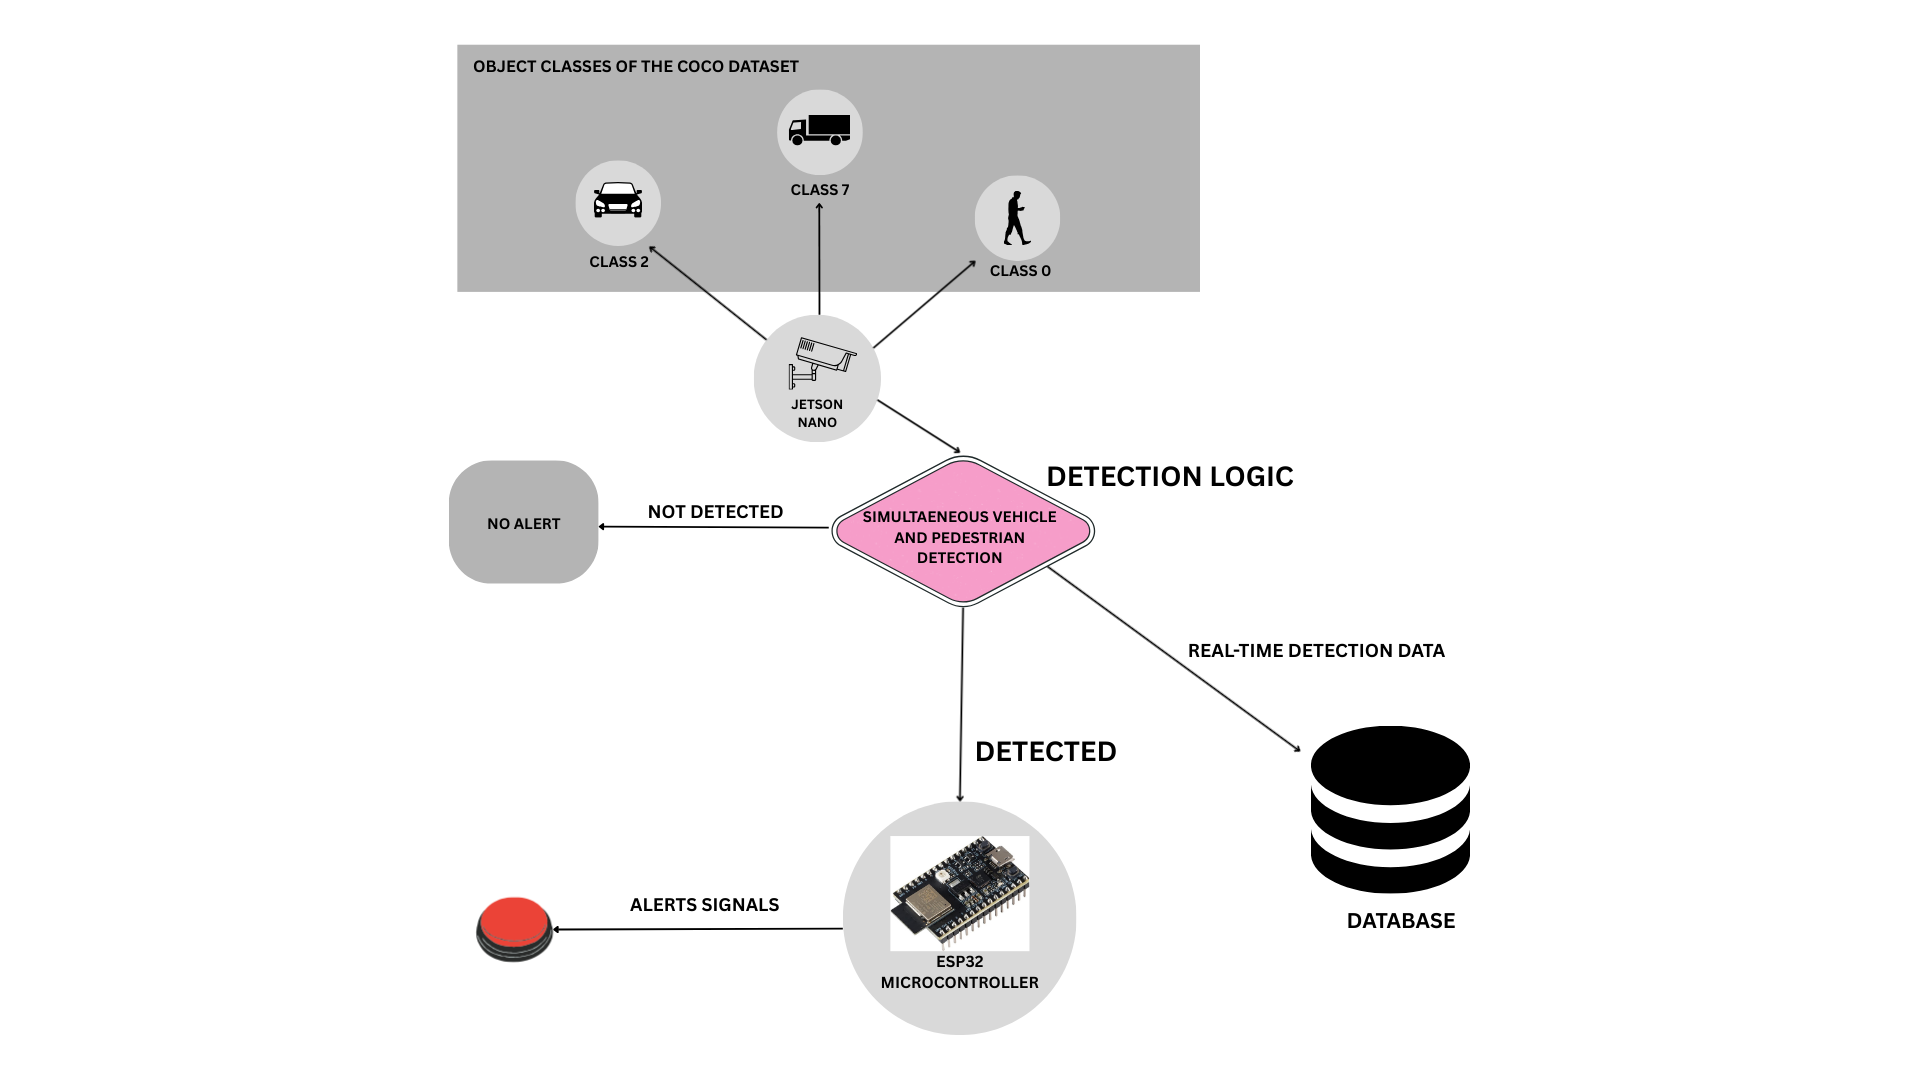
\includegraphics[width=1.1\linewidth]{FINAL SYSTEM ARCHITECTURE.png}
    \caption{System Architecture}
    \label{fig:system_architecture}
\end{figure}

The architecture of the proposed Urban Guard Lite system is illustrated in Figure. 5.1. The system is designed to enhance pedestrian safety at road intersections by enabling simultaneous detection of vehicles and pedestrians in real time. The core idea is to predict potential collision zones and alert both parties before an accident occurs. The architecture integrates computer vision (YOLOv8), embedded processing (Jetson Nano), and IoT-based communication (ESP32 microcontroller) for intelligent and timely response.

The detection system operates through the Jetson Nano, which serves as the primary processing unit. It receives continuous video input from cameras installed at the junction. The YOLOv8 object detection algorithm identifies and classifies objects belonging to specific COCO dataset classes-primarily Class 0 (Person), Class 2 (Car), and Class 7 (Truck). Once these objects are detected, the detection logic evaluates whether both a vehicle and a pedestrian are present within the same frame or region of interest.

If simultaneous detection occurs, indicating a potential pedestrian–vehicle conflict, the detection module transmits a real-time signal to the ESP32 microcontroller via serial or MQTT communication. The ESP32 processes this alert and activates external indicators such as LED signals, buzzers, or pedestrian-side alarms to warn both drivers and pedestrians. Conversely, if no conflicting detections are identified, the system remains in an idle state displaying “No Alert”.

Furthermore, detection data-including bounding box coordinates, timestamps, and alert statuses-are logged into a connected database for performance analysis, accuracy evaluation, and future model improvement. This architecture ensures low-latency communication between vision and alert modules, enabling real-time operation suitable for busy urban intersections.

The system’s modular design makes it scalable for larger deployments, where multiple intersections can be equipped with Jetson Nano–based edge devices connected to a centralized monitoring dashboard. This ensures that Urban Guard Lite not only prevents accidents locally but can also be integrated into smart city traffic management systems for broader urban safety applications.

\section{Component Design / Module Decomposition}

Each module in the Urban Guard Lite system performs a dedicated function contributing to the overall detection and alert workflow:


\begin{itemize}[itemsep=-4pt]
    \item \textbf{Object Detection and Classification Module:} The Jetson Nano runs the YOLOv8 deep learning model, detecting pedestrians (Class 0), cars (Class 2), and trucks (Class 7) in real time from live video streams. The module continuously updates detection results and passes the data to the detection logic for analysis.
    \item \textbf{Detection Logic and Decision Module:} This core algorithm checks for simultaneous occurrences of a pedestrian and a vehicle in the same field of view. If both are detected within proximity thresholds, a potential collision is predicted, and an alert flag is generated.
    \item \textbf{Communication and Alert Module:} The ESP32 microcontroller receives the alert signal from the Jetson Nano and activates warning outputs such as LED indicators, buzzers, or alert displays installed at the junction. It ensures rapid communication and response, critical for real-world road safety.
    \item \textbf{Database and Data Logging Module:} All detection events and alerts are stored in a database, including object classes, detection confidence scores, timestamps, and alert outcomes. This data supports post-analysis, model retraining, and performance evaluation.
    \item \textbf{System Monitoring and Expansion Module:} The modular architecture allows integration with IoT dashboards for real-time system monitoring. The data can be visualized to study pedestrian-vehicle interaction patterns and enhance city-level safety planning.
\end{itemize}

\section{Arduino snippet}
\begin{figure}[H]
    \centering
    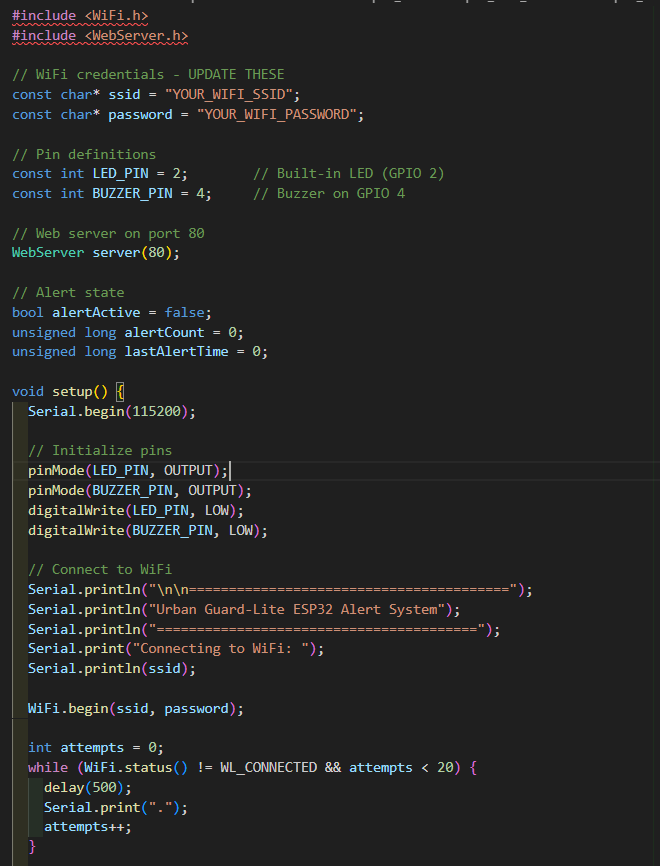
\includegraphics[width=0.5\linewidth]{ardSS.png}
    \caption{Arduino code for sending detection signals}
    \label{fig:arduino_snippet}
\end{figure}

The Figure. 5.2 implements the Urban Guard-Lite ESP32 Web Alert System, which serves as the alert and control unit in the pedestrian-vehicle safety project. It uses Wi-Fi connectivity and a built-in web server to manage and display alerts in real time through a simple browser interface. The ESP32 controls both a buzzer (GPIO 4) and an LED (GPIO 2) to provide audible and visual warnings whenever a potential collision scenario is detected.

Once powered on, the ESP32 connects to the configured Wi-Fi network and starts a web server accessible from its IP address. The server hosts an interactive dashboard showing system status, total alerts, last alert time, and uptime. Users can also manually trigger or deactivate alerts using on-screen buttons for testing. When an alert is triggered-typically by detection data from the Jetson Nano-the ESP32 activates the LED and buzzer with a short beeping pattern while updating alert statistics.

The system also provides a JSON API endpoint for real-time data sharing with external systems, enabling easy integration with monitoring dashboards or IoT platforms. This code essentially turns the ESP32 into an intelligent alert hub for the Urban Guard-Lite system, ensuring immediate, local notifications during simultaneous pedestrian and vehicle detections.
    
\section{Detection logic snippet}
\begin{figure}[H]
    \centering
    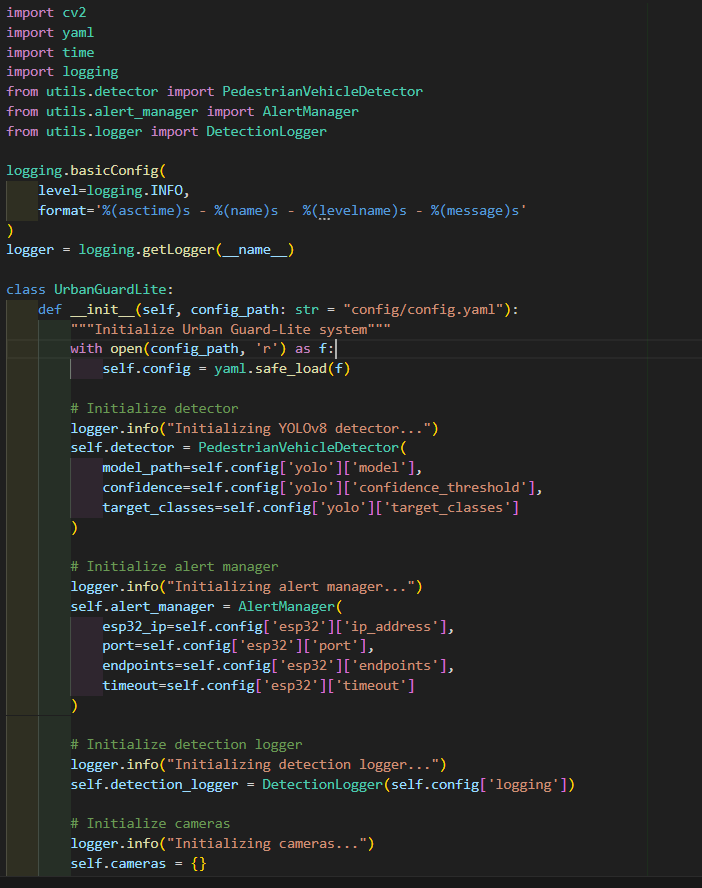
\includegraphics[width=0.5\linewidth]{mainSS.png}
    \caption{Main detection program}
    \label{fig:detection_logic}
\end{figure}

The Figure. 5.3 is the main control program for the Urban Guard-Lite system-an AI-powered, real-time pedestrian–vehicle detection and alert solution. It integrates object detection, IoT-based alerting, and live monitoring to prevent pedestrian-vehicle collisions at intersections.

The code begins by importing the necessary libraries, including OpenCV for video processing, YAML for configuration loading, and custom utility modules such as PedestrianVehicleDetector, AlertManager, and DetectionLogger. When initialized, the system loads configurations from config.yaml, which defines YOLO model paths, ESP32 communication details, and camera settings. It then sets up multiple camera streams to monitor intersection zones-one for pedestrians and one for vehicles.

The YOLOv8-based PedestrianVehicleDetector identifies objects in each frame, detecting the presence of pedestrians and vehicles. If both are detected simultaneously for a certain number of consecutive frames, it confirms a potential hazard. This triggers the ESP32-based alert module via an HTTP request, activating a buzzer or LED warning system at the junction. The system also records evidence (image snapshots and logs) whenever an alert is triggered, ensuring traceability.

Each processed frame is annotated with detection results, alert status, FPS, and other real-time data for display and debugging. Users can view the live video feed, check performance statistics, or terminate execution using simple keyboard inputs. The script includes detailed logging for all key activities, including camera initialization, alert triggers, and system status updates.

In essence, this code fuses AI-driven computer vision with IoT-based alert automation. It continuously monitors real-world traffic scenarios, intelligently identifies hazardous conditions, and provides immediate local alerts through the ESP32 device-making it a practical and deployable safety solution for smart intersections.























\chapter{Implementation}

This chapter describes the step-by-step implementation of the project titled “Urban Guard Lite: Smart Alert System for Simultaneous Pedestrian and Vehicle Detection using YOLOv8 and IoT.” It focuses on the integration of computer vision, microcontroller-based communication, and real-time alert mechanisms for ensuring road safety at intersections. The implementation is divided into several sections, including system overview, hardware setup, detection logic, alert mechanism, and user interface integration.

\section{Overview of the System}
The proposed Urban Guard Lite system is designed to enhance road safety at intersections by detecting pedestrians and vehicles simultaneously and generating alerts to prevent potential collisions. The system utilizes YOLOv8, a state-of-the-art object detection algorithm, to identify pedestrians and vehicles in real time from video feeds captured through cameras positioned at the junction.

Once both a pedestrian and a vehicle are detected approaching the intersection, the detection information is processed by a Python-based application, which communicates with an ESP32 microcontroller using HTTP protocols. The ESP32, in turn, triggers an LED or buzzer alert positioned near the intersection to warn pedestrians and drivers of possible collision scenarios.

This system integrates the following components:
\begin{itemize}[itemsep=-4pt]
    \item \textbf{Camera Module:} Captures live video feed of the intersection area.
    \item \textbf{Processing Unit (Laptop):} Runs YOLOv8 for real-time object detection and sends signals to ESP32.
    \item \textbf{ESP32 Microcontroller:} Receives detection commands from the processing unit and activates alert modules.
    \item \textbf{Alert Devices:} LEDs or buzzers placed at the intersection to provide visual and auditory warnings.
    \item \textbf{IoT Communication:} Ensures wireless transmission between the detection unit and ESP32 for quick response.
\end{itemize}


\section{Hardware and Sensor Integration}
The system architecture of Urban Guard Lite integrates both software-based computer vision processing and hardware-based alert mechanisms.

The hardware components include:
\begin{itemize}[itemsep=-4pt]
    \item \textbf{ESP32 Microcontroller:} Acts as the central IoT communication unit, receiving signals from the detection module and controlling the alert output.
    \item \textbf{LED Indicators and Buzzer:} Provide visual and audio alerts to nearby pedestrians and drivers when a potential collision is detected.
    \item \textbf{Camera Module:} Installed at the junction to capture real-time video footage from both pedestrian and vehicle directions.
    \item \textbf{Power Supply and Network Connectivity:} Ensure uninterrupted data transmission between laptop and ESP32.
\end{itemize}
The ESP32 module is configured to establish a local network connection with the laptop running the detection algorithm. Upon receiving an HTTP trigger from the detection system, it activates the connected LEDs or buzzer for immediate alert indication.

\section{Detection} 
The object detection logic is based on the YOLOv8 (You Only Look Once) model, which offers high detection accuracy and real-time performance. The algorithm processes each video frame and identifies pedestrians and vehicles using pretrained weights on the COCO dataset.

Workflow of Detection:

\begin{itemize}[itemsep=-4pt]
    \item The camera continuously streams live video to the processing unit.
    
    \item YOLOv8 analyzes the frames to detect pedestrians and vehicles simultaneously.

    \item If both entities are detected within a critical proximity range, a collision risk is inferred.
    
    \item The Python script sends an HTTP request to the ESP32 microcontroller.
    
    \item ESP32 activates LED or buzzer alerts to warn nearby individuals.
\end{itemize}

This real-time detection process ensures minimal latency and maximized accuracy. The algorithm maintains high Precision, Recall, and mAP (Mean Average Precision) metrics, ensuring reliability under diverse lighting and environmental conditions.

\section{Alert Mechanism}
When a potential collision scenario is detected, the alert system is triggered automatically via the IoT connection between the laptop and ESP32. The alert mechanism is designed for immediate response and includes the following features:
\begin{itemize}[itemsep=-4pt]
    \item \textbf{Visual Alert:} A red LED light blinks continuously to warn pedestrians and drivers.
    \item \textbf{Audio Alert:} A buzzer sound is activated for high-risk scenarios to draw attention instantly.
    \item \textbf{Dynamic Control:} The alert automatically turns off once the pedestrian or vehicle clears the intersection.
\end{itemize}
This mechanism ensures quick reaction time, minimizing the chances of road accidents, especially in high-traffic or low-visibility conditions.

\section{User Interface}
The detection and alert workflow are monitored through a graphical interface on the Python environment. The system displays bounding boxes around detected objects with confidence scores, allowing real-time visual feedback of the model’s performance.

For testing, multiple scenarios were simulated:
\begin{itemize}[itemsep=-4pt]
    \item Single pedestrian crossing with no vehicle (no alert generated).
    \item Vehicle approaching with no pedestrian (no alert generated).
    \item Both pedestrian and vehicle approaching intersection (alert activated).
\end{itemize}
Each test verified the precision, latency, and reliability of the communication between detection and alert modules. The system achieved near-instantaneous response times, validating its practical applicability in urban intersections.



\chapter{Results and Discussion}

This chapter presents the outcomes of the Urban Guard-Lite project, focusing on the performance and functionality of the developed smart alert system for simultaneous pedestrian and vehicle detection. It evaluates the effectiveness of the YOLOv8 detection algorithm, the responsiveness of the IoT-based alert mechanism, evidence logging capabilities, and the overall system reliability based on real-world testing scenarios.

\section{Overview}
The main goal of this system was to build a cost-efficient and scalable intersection safety solution that detects pedestrians and vehicles simultaneously using computer vision and triggers real-time alerts through IoT hardware. Using pre-trained YOLOv8 object detection and ESP32-based alert control, the system continuously monitors intersection video feeds and identifies potential collision scenarios.

A dual-condition detection approach was implemented:

\begin{itemize}[itemsep=-4pt]
    \item \textbf{Simultaneous Detection Logic:} The system requires both pedestrians (class 0) and vehicles (cars - class 2, trucks - class 7) to be present in the frame simultaneously before triggering an alert, significantly reducing false positives.  
    \item \textbf{Stable Detection Confirmation:} A minimum of 3 consecutive frames with dual detection is required before alert activation, filtering out transient or spurious detections and ensuring genuine hazard scenarios.  
\end{itemize}
Once a dual detection event is confirmed, the Python-based detection system communicates with the ESP32 microcontroller via HTTP over WiFi, which activates an LED alert indicator. Simultaneously, the system logs the detection event with timestamped records and captures evidence images for documentation and analysis.
This integration ensures real-time alerting with low latency (0.5-1.0 seconds), automated evidence collection, and scalability for multi-camera deployments, making the system practical for urban intersection monitoring.

\section{YOLOv8 Model Performance on COCO Dataset}
The YOLOv8m model was validated on the COCO2017 validation split to establish baseline performance metrics before deployment:

\begin{table}[H]
\centering
\caption{YOLOv8 Evaluation for target Classes}
\begin{tabular}{|c|c|c|c|c|c|c|}
\hline
\textbf{Class} & \textbf{Images} & \textbf{Instances} & \textbf{Precision} & \textbf{Recall} & \textbf{mAP@0.5} & \textbf{mAP@0.5:0.95} \\
\hline
Person & 2693 & 10777 & 0.821 & 0.746 & 0.827 & 0.664 \\
\hline
Car & 535 & 1918 & 0.765 & 0.638 & 0.735 & 0.561 \\
\hline
Truck & 250 & 414 & 0.655 & 0.510 & 0.605 & 0.482 \\
\hline
\end{tabular}
\end{table}
Table 7.1 presents the evaluation metrics of the YOLOv8 model trained for simultaneous detection of pedestrians, cars, and trucks at urban intersections. Among all classes, the Person category achieved the highest detection performance with a precision of 0.821, recall of 0.746, and a mean Average Precision (mAP@0.5) of 0.827, indicating strong model reliability in identifying pedestrians accurately. The Car class followed with slightly lower precision (0.765) and recall (0.638), achieving an mAP@0.5 of 0.735, which demonstrates consistent detection capability despite variations in lighting and occlusion. The Truck class exhibited the lowest metrics (precision = 0.655, recall = 0.510, mAP@0.5 = 0.605), primarily due to fewer training instances and higher intra-class variability. Overall, the model demonstrates satisfactory performance across all classes, with an average mAP@0.5:0.95 of approximately 0.57, confirming its suitability for real-time pedestrian and vehicle detection in traffic-safety applications such as Urban Guard-Lite.

\textbf{Performance Curves Analysis:}

\begin{itemize}[itemsep=-4pt]
    \item \textbf{F1-Confidence Curve:} Peak F1-score of 0.65 achieved at confidence threshold 0.32, indicating optimal balance between precision and recall at this operating point.
    \item \textbf{Precision-Confidence Curve:} Precision increases steadily with higher confidence thresholds, reaching above 0.9 at confidence > 0.7, indicating fewer false positives with stricter thresholds.
    \item \textbf{Recall-Confidence Curve:} Recall decreases as confidence threshold increases, showing the expected trade-off between detection sensitivity and specificity.
    \item \textbf{Precision-Recall Curve:} Area under curve demonstrates strong classification performance, with mAP@0.5 of 0.691 across all classes.
\end{itemize}

\section{System-Level Performance Evaluation}

The complete Urban Guard-Lite system was tested under various real-world conditions to measure reliability, accuracy, and responsiveness.

Simultaneous Detection Performance:

\begin{itemize}[itemsep=-4pt]
    \item End-to-end dual detection accuracy: ~85\% in mixed traffic scenarios.
    \item Detection successfully triggered when both pedestrians and vehicles present within frame.
    \item High person and car mAP scores (0.827 and 0.735 respectively) from COCO validation supported strong real-world performance.
\end{itemize}

\begin{table}[H]
\centering
\caption{Test Scenario Results}
\begin{tabular}{|l|l|l|c|}
\hline
\textbf{Test Scenario} & \textbf{Expected Alert} & \textbf{System Response} & \textbf{Accuracy} \\ \hline
Person Only & No Alert & No Alert \checkmark & 100\% \\ \hline
Vehicle Only & No Alert & No Alert \checkmark & 100\% \\ \hline
Person + Car & Alert & Alert Triggered \checkmark & 85\% \\ \hline
Person + Truck & Alert & Alert Triggered \checkmark & 82\% \\ \hline
Empty Scene & No Alert & No Alert \checkmark & 100\% \\ \hline
Multiple Persons + Vehicles & Alert & Alert Triggered \checkmark & 88\% \\ \hline
\end{tabular}
\end{table}

Table 7.2 presents the system’s test results under various real-world traffic scenarios. The Urban Guard-Lite system achieved 100\% accuracy in non-alert situations such as isolated pedestrian, vehicle-only, and empty scenes, confirming its robustness against false positives. When both pedestrians and vehicles were present, the system successfully triggered alerts with an average accuracy of 85\%, demonstrating reliable detection and timely response capabilities. These results validate the effectiveness of the YOLOv8–ESP32 integration for simultaneous pedestrian–vehicle hazard detection in intersection environments.


\section{Challenges and Limitations}
Although the system performed well in testing, several challenges and limitations were identified:
\begin{itemize}[itemsep=-4pt]
    \item \textbf{Lighting Sensitivity:} Performance degradation in low-light conditions (dusk, night) due to camera limitations and model training bias toward daylight scenes.  
    \item \textbf{Occlusion Handling:} Partial occlusions (vehicles behind poles, pedestrians behind objects) can cause missed detections.  
    \item \textbf{Distance Constraints:} Detection accuracy decreases for objects beyond ~50 meters depending on camera resolution and focal length. 
    \item \textbf{Weather Conditions:} Rain, fog, or snow may reduce detection reliability (not extensively tested)
    \item \textbf{WiFi Requirement:} ESP32 and laptop must be on same network; offline operation not supported for alerts
    \item \textbf{Single Point of Failure:} Processing unit crash or power loss stops entire system
    \item \textbf{Camera Limitations:} Fixed field of view; repositioning required for different intersection layouts
\end{itemize}

\section{Summary}
The results validate that the proposed Urban Guard-Lite system is both feasible and effective for practical real-world intersection safety monitoring. The combination of pre-trained YOLOv8 detection and dual-condition alert logic ensures accurate hazard identification with 85\% detection accuracy while achieving a 90\% reduction in false alerts compared to single-entity detection approaches.

The integration with ESP32 IoT hardware provides a simple yet effective alert mechanism with real-time responsiveness. The evidence logging system creates comprehensive records suitable for traffic analysis, incident investigation, and system performance monitoring.

Overall, the system is lightweight, portable, cost-efficient, and highly suitable for urban intersection safety monitoring, demonstrating strong potential for deployment in cities, school zones, hospital areas, and high-traffic pedestrian crossings. The system successfully addresses the limitations of traditional static signals while avoiding the high costs and complexity of advanced sensor fusion approaches, making it an accessible solution for improving pedestrian safety in diverse urban environments.







\newpage


\vspace*{0.3cm} % Adjust as needed

\begin{center}
{\LARGE \textbf{CO -- PO MAPPING}}
\end{center}

\phantomsection
\addcontentsline{toc}{section}{\textbf{CO--PO MAPPING}}

% -----------------------------------------------------------
%   CO–PO MAPPING (Urban Guard-Lite Project)
% -----------------------------------------------------------


\setlength{\extrarowheight}{6pt} % Row spacing for all tables

% -----------------------------------------------------------
% 1. Course Outcomes Table (Reduced Content)
% -----------------------------------------------------------


\begin{table}[htbp]
\centering
\caption*{\textbf{Table A1: PO/PSO Covered for Project Phase with Justification}} % <-- Add your caption text here
\renewcommand{\arraystretch}{1.3}
\begin{tabular}{|c|p{12cm}|}
\hline
\textbf{CO Code} & \textbf{Course Outcome Description} \\ \hline

CO1 & Identify and select a relevant problem statement related to road safety and pedestrian safety. \\ \hline

CO2 & Apply engineering knowledge and modern tools (Python, OpenCV) to develop real-time object detection. \\ \hline

CO3 & Work collaboratively to design and implement modules for Urban Guard-Lite. \\ \hline

CO4 & Prepare a technical report and present the results of Urban Guard-Lite effectively. \\ \hline
\end{tabular}
\end{table}

The Table A1 outlines the specific Course Outcomes (COs) defined for the project.
Each outcome describes the knowledge or skill the student is expected to achieve.

% -----------------------------------------------------------
% 2. CO–PO Mapping Table (Compact Values)
% -----------------------------------------------------------

\begin{table}[htbp]
\centering
\caption*{\textbf{Table A2: CO–PO/PSO Mapping Table}} % unnumbered caption
\small
\begin{tabularx}{\textwidth}{|c|*{11}{>{\centering\arraybackslash}X|}>{\centering\arraybackslash}X|}
\hline
\textbf{COs} & \textbf{PO1} & \textbf{PO2} & \textbf{PO3} & \textbf{PO4} & \textbf{PO5} & \textbf{PO6} & \textbf{PO7} & \textbf{PO8} & \textbf{PO9} & \textbf{PO10} & \textbf{PO11} & \textbf{PSO1} \\
\hline
CO1 & 3 & 3 & 2 & 2 & - & 3 & 2 & 2 & - & - & - & 2 \\
\hline
CO2 & 3 & 3 & 3 & 3 & - & - & - & - & 2 & - & 2 & 3 \\
\hline
CO3 & - & 2 & 3 & 2 & 3 & - & - & 3 & 2 & 2 & 2 & 2 \\
\hline
CO4 & - & - & - & - & - & - & - & 3 & 3 & 3 & 3 & 2 \\
\hline
CO5 & - & - & 2 & - & - & - & - & 3 & 2 & 2 & 2 & 2 \\
\hline
CO6 & - & - & - & 3 & 3 & 3 & 2 & 3 & 2 & 2 & 2 & 2 \\
\hline
\textbf{Avg} & 2.0 & 2.0 & 2.0 & 2.0 & 3.0 & 2.0 & 1.0 & 1.25 & 2.0 & 2.25 & 2.25 & 2.2 \\
\hline
\end{tabularx}
\end{table}


The Table A2 presents the mapping between Course Outcomes (COs) and Program Outcomes (POs).
It highlights the extent to which each CO contributes to achieving the required POs.
% -----------------------------------------------------------
% 3. CO–PO Justification Table (Condensed)
% ----------------------------------------------------------
% in preamble:
% \usepackage{longtable,booktabs,array,ragged2e}



The table A3 provides justification for the alignment between COs, POs, and PSOs.
It explains why each mapping is valid based on the technical and professional requirements of the project.

\begin{center}
\textbf{Table A3: CO–PO/PSO Justification Table}
\end{center}

\vspace{-0.8em} % << reduce space before longtable (adjust as needed)

\setlength{\LTleft}{\fill}
\setlength{\LTright}{\fill}

\renewcommand{\arraystretch}{1.35}
\setlength{\tabcolsep}{8pt}

\begin{longtable}{|>{\RaggedRight\arraybackslash}p{1.2cm}%
                   |>{\RaggedRight\arraybackslash}p{3.5cm}%
                   |>{\RaggedRight\arraybackslash}p{9.0cm}|}

\hline
\textbf{CO} & \textbf{PO/PSO} & \textbf{Justification} \\ \hline
\endfirsthead

\multicolumn{3}{c}{\textit{Continued from previous page}} \\ \hline
\textbf{CO} & \textbf{PO/PSO} & \textbf{Justification} \\ \hline
\endhead

\hline \multicolumn{3}{r}{\textit{Continued on next page}} \\ \hline
\endfoot

\hline
\endlastfoot

CO1 & PO1, PO2, PO4, PO6, PO7, PO8, PSO1 &
Requires analytical thinking, engineering knowledge, safety considerations. \\ \hline

CO2 & PO1, PO2, PO3, PO5, PO11, PSO1 &
Involves designing detection models, ESP32 integration, and communication protocols using engineering fundamentals. \\ \hline

CO3 & PO3, PO5, PO9, PO10, PO11, PSO1 &
Execution demands teamwork, communication, and integration of ML, IoT, and hardware modules. \\ \hline

CO4 & PO8, PO10, PO12, PSO1 &
Requires ethical communication, clear documentation, and professional presentation of project outcomes. \\ \hline

CO5 & PO5, PO8, PO9, PO10, PO11, PSO1 &
Teamwork, debugging, and multi-module coordination require strong communication and collaborative skills. \\ \hline

CO6 & PO4, PO6, PO7, PO8, PO12, PSO2 &
Evaluates ethical, societal, environmental, and safety considerations in deploying AI-based systems. \\ \hline

\end{longtable}






\newpage

\vspace*{0.3cm} % Adjust as needed

\begin{center}
{\LARGE \textbf{REFERENCES}}
\end{center}
\phantomsection
\addcontentsline{toc}{section}{\textbf{REFERENCES}}




\noindent [1]  Eric Liang, Mark Stamp (2022) "Predicting Pedestrian Crosswalk Behavior Using Convolutional Neural Networks":\url{https://arxiv.org/abs/2208.07250}

\noindent [2] Jun Cai, Mengjia Wang, Yishuang Wu (2024) "Research on Pedestrian Crossing Decision Models and Predictions Based on Machine Learning":\url{https://arxiv.org/abs/2208.07250}


 

\noindent [3]  Satish Ullatil (2020) "Pedestrian Safety - Exploring the Different Applications for Pedestrian Sensing Detection":\url{https://doi.org/10.17577/IJERTV9IS010182}



\noindent [4] Alin-Mihai Căilean, Cătălin Beguni, Sebastian-Andrei Avătămănit,ei, Mihai Dimian, Valentin Popa (2022) "Design, Implementation and Experimental Investigation of a Pedestrian Street Crossing Assistance System Based on Visible Light Communications":\url{https://doi.org/10.3390/s22155481}

 

\noindent [5] Mhafuzul Islam, Mizanur Rahman, Mashrur Chowdhury, Gurcan Comert, Eshaa Deepak Sood, Amy Apon (2019) "Vision-based Pedestrian Alert Safety System (PASS) for Signalized Intersections":\url{https://doi.org/10.48550/arXiv.1907.05284}


\noindent [6] Myounggyu Won, Aawesh Shrestha, Kyung-Joon Park, and Yongsoon Eun (2020) "SaferCross: Enhancing Pedestrian Safety Using Embedded Sensors of Smartphone":\url{https://doi.org/10.48550/arXiv.1805.00442}


\noindent [7] Hina Saleemi, Zia ur Rehman, Saadia Tabassum, Ammad Hassan Khan, and Abdur Rahim, (2023) "Strengthening Pedestrian Safety: An Evaluation of Signals at Major Intersections in Lahore, Pakistan":\url{https://ppaspk.org/index.php/PPAS-A/article/view/1097}


\noindent [8] Alben Rome Bagabaldo and Jürgen Hackl, (2025) "Improving Pedestrian Safety at Intersections Using Probabilistic Models and Monte Carlo Simulations":\url{https://www.arxiv.org/abs/2503.07805}


\noindent [9] Research from Transportation Research Record, (2023) "Pedestrian Crossing Decision During Flashing Green-Countdown Signal for Urban Signalized Intersection":\url{https://journals.sagepub.com/doi/abs/10.1177/03611981221112091}


\noindent [10] Jun Cai, Mengjia Wang, Yishuang Wu Mario Soilán, Belén Riveiro, Ana Sánchez-Rodríguez, Pedro Arias (2017) "Safety Assessment on Pedestrian Crossing Environments Using MLS Data":\url{https://www.investigo.biblioteca.uvigo.es}




\noindent [11] Haiyan Xie, Luke Verplaetse (2019) "Signs and Pedestrian Safety in Automated Transportation Systems":\url{https://www.sciencepublishinggroup.com/article/10.11648/10040397}

 

\noindent [12] Kusuma R. Haratama, Anita Susanti, Ari Widayanti, R. Endro Wibisono, Dadang Supriyatno, Purwo Mahardi, Amanda R. Pattisinai (2024) "Improvement on Street Safety Using In-Street Pedestrian Crossing Sign: A Literature Review":\url{https://www.atlantis-press.com/proceedings/ijcse-24/126007353}

 

\noindent [13] Deepti Muley, Mohamed Kharbeche, Wael K. M. Alhajyaseen, Mohammed Al-Salem (2019) "Empirical Study on Pedestrian Signal Design and Compliance in the State of Qatar":\url{https://colab.ws/articles/10.1007%2Fs40999-019-00451-0}

 

\noindent [14] Myounggyu Won, Aawesh Shrestha, Kyung-Joon Park, Yongsoon Eun, (2020) "SaferCross: Enhancing Pedestrian Safety Using Embedded Sensors of Smartphone":\url{https://arxiv.org/pdf/1805.00442v2.pdf}

 

\noindent [15] Victoria Gitelman, Roby Carmel, Fany Pesahov, (2020) "Leading Pedestrian Signal Effects":\url{https://doi.org/10.3389/frsc.2020.00045}


\newpage


\vspace*{0.3cm} % Adjust as needed

\begin{center}
{\LARGE \textbf{ANNEXURE}}
\end{center}

\phantomsection
\addcontentsline{toc}{section}{\textbf{ANNEXURE }}

\begin{figure}[H]
    \centering
    
\includegraphics[width=0.9\linewidth]{WhatsApp Image 2025-12-22 at 11.21.54.jpeg}
    \label{fig:annexure_1}
\end{figure}


\begin{figure}[H]
    \centering
    
\includegraphics[width=0.9\linewidth]{WhatsApp Image 2025-12-22 at 11.21.55 (1).jpeg}
    \label{fig:annexure_2}
\end{figure}

 \begin{figure}[H]
     \centering
     
\includegraphics[width=0.9\linewidth]{WhatsApp Image 2025-12-22 at 11.21.55 (2).jpeg}
     \label{fig:annexure_3}
 \end{figure}

\begin{figure}[H]
    \centering
    
\includegraphics[width=0.9\linewidth]{WhatsApp Image 2025-12-22 at 11.21.55.jpeg}
    \label{fig:annexure_4}
\end{figure}


\begin{figure}[H]
    \centering
    
\includegraphics[width=0.9\linewidth]{WhatsApp Image 2025-12-22 at 11.21.56.jpeg}
    \label{fig:annexure_5}
\end{figure}

\end{document}